\chapter{Wprowadzenie teoretyczne}
W poniższym rozdziale omówiona zostanie krótko historia badań nad interpretowalnością sieci neuronowych. W szczególności analiza, w tym kontekście, sieci konwolucyjnych (ang. \textit{Convolutional Neural Networks}). Przybliżona zostanie także architektura sieci typu transformer oraz jej rola w modelach językowych. W dalszej części opisana zostanie literatura skupiająca swoją uwagę na badaniu interpretowalności modeli językowych oraz rola Rzadkich Autoenkoderów (ang. \textit{Sparse Autoencoders}) w ekstrakcji cech. Na koniec omówione zostaną modele typu MoE (ang. \textit{Mixture of Experts}), sposoby ich budowania oraz możliwość zastosowania w owej pracy.

\section{Interpretowalność sieci neuronowych}
\label{sec:interpretowalnosc_sieci_neuronowych}
Sieci neuronowe zbudowane są ze sztucznych neuronów -- prostej jednostki przetwarzającej wartości otrzymane na wejściu od połączonych z nią neuronów i produkującej na wyjściu wartość swojego pobudzenia. Każdy neuron przypisuje do każdego innego połączonego z nim neuronu wagę, posiada własny parametr przesunięcia (ang. \textit{bias}) oraz nieliniową funkcję aktywacji. Mnożąc każde wejście przez odpowiadającą mu wagę, następnie dodając wartość przesunięcia i na koniec stosując funkcję aktywacji, dostaje na wyjściu liczbę, która jest wartością jego aktywacji. W sieciach neuronowych, zwłaszcza w większych modelach, połączonych ze sobą w warstwy są miliony, lub nawet miliardy neuronów. Każdy neuron aktywuje się w odpowiedzi na inny sygnał lub zestaw sygnałów, a grupy neuronów przetwarzających sygnały w podobny do siebie sposób są rozproszone po całej sieci. Cały ten szereg komplikacji sprawia, że nie da się w prosty i jednoznaczny sposób odpowiedzieć na pytania dlaczego sieć dała konkretną odpowiedź, lub jaki proces doprowadził do danego wyniku. \newline
Powstało wiele podejść tworzenia i badania mechanizmów wyjaśniających sposoby działania złożonych modeli. Zgodnie z podziałem literatury w artykule przeglądowym autorstwa Tilmana Räukera \cite{rauker_toward_transparent_ai}, tradycyjne podejścia w ramach wyjaśnialnej sztucznej inteligencji (ang. \textit{Explainable AI}) opierają się głównie na metodach post-hoc, które traktują model jak czarną skrzynkę. Metody te próbują wyjaśnić decyzje modelu na podstawie analizy jego wejść i wyjść, odpowiadając m.in. na pytanie jakie próbki lub cechy w najbardziej znaczący sposób wpływają na wynik modelu. Pomaga to zrozumieć zależności przyczynowo-skutkowe pomiędzy danymi wejściowymi a wynikami modelu. W opozycji do tego stoi poddziedzina nazywana mechanistyczną interpretowalnością (ang. \textit{mechanistic interpretability}), które skupia się na wewnętrznej strukturze modelu. To podejście wykorzystuje proces inżynierii odwrotnej sieci neuronowej na poziomie pojedynczych neuronów i ich połączeń. Pozwala to zrozumieć wewnętrzną logikę i mechanikę działania modelu. Odpowiada na pytanie w jaki sposób jego poszczególne komponenty (takie jak węzły i wagi w modelach głębokich sieci neuronowych) generują odwzorowanie pomiędzy danymi wejściowymi a wynikiem działania systemu. \newline
Niniejsza praca w przeważającej większości korzysta z podejścia mechanistycznego. Wybór ten wynika z ograniczeń, jakie niesie ze sobą klasyczne podejście post-hoc. Cynthia Rudin w pracy \cite{rudin_stop_explaining_black_box_machine_learning_models} argumentuje, że wyjaśnienia nakładane na czarną skrzynkę po fakcie są jedynie przybliżeniem rzeczywistego działania modelu -- gdyby odwzorowywały je w pełni wiernie, same stałyby się tym modelem, co czyni je z definicji częściowo niedokładnymi. W kontekście decyzji o wysokiej stawce, w obliczu jakich stawia się obecnie modele sztucznej inteligencji, tj. diagnozy medyczne czy wyroki sądowe, wymagana jest większa wierność wyjaśnianych elementów. Mechanistyczna interpretowalność podąża inną drogą: próbuje wiernie zrekonstruować mechanizm, który już wewnątrz sieci istnieje. Ponieważ opiera się na bezpośredniej analizie wag i aktywacji, a nie na przybliżeniach formułowanych wyłącznie na podstawie wejść i wyjść, pozwala uniknąć problemu utraty wierności. \newline
Szersze motywacje stojące za potrzebą interpretowalności -- obejmujące zarówno bezpieczeństwo systemów sztucznej inteligencji, jak i możliwości optymalizacji architektur -- zostały omówione w rozdziale~\ref{sec:motywacja}; tu wystarczy zaznaczyć, że mechanistyczna interpretowalność odpowiada na nie w sposób, którego podejście post-hoc z definicji nie może zapewnić.


\section{Wczesne prace nad wizualizacją i interpretacją głębokich sieci neuronowych} 
\label{sec:wczesne_prace_wizualizacja}
W 2006 roku Geoffrey Hinton wraz ze współpracownikami opublikował dwa przełomowe artykuły, które zapoczątkowały tzw. renesans głębokiego uczenia (ang. \textit{deep learning}). Wykazano w nich, że wielowarstwowe sieci neuronowe -- dotąd trudne do skutecznego trenowania metodą propagacji wstecznej ze względu na problem zanikającego gradientu i słabą jakość znajdywanych minimów -- można efektywnie uczyć dzięki wstępnemu, nienadzorowanemu trenowaniu warstwa po warstwie z wykorzystaniem Maszyn Boltzmanna z ograniczeniami (ang. \textit{Restricted Boltzmann Machines, RBMs}) \cite{hinton_reducing_the_dimensionality_of_data} \cite{hinton_a_fast_learning_algorithm_for_deep_belief_nets}. Niemal równolegle analogiczną, zachłanną metodę wstępnego trenowania, opartą na autoenkoderach, rozwijał zespół Yoshuy Bengio \cite{lamblin_greedy_layer_wise_training_of_deep_networks}. \newline
Sukces w trenowaniu głębokich architektur postawił nowe pytanie badawcze: co właściwie poszczególne warstwy sieci uczą się reprezentować? Dotychczasowe prace poświęcone interpretacji sieci neuronowych ograniczały się zasadniczo do pierwszej warstwy, której wagi -- traktowane jako filtry w przestrzeni wejściowej -- dawało się przedstawić w postaci obrazów przypominających m.in. detektory krawędzi lub filtry Gabora. Interpretacja warstw głębszych pozostawała znacznie trudniejsza, ponieważ ich reprezentacji nie można było odczytać w równie bezpośredni sposób. \newline
Pierwsze próby wyjścia poza pierwszą warstwę podjęli Honglak Lee i współpracownicy, którzy -- opierając się na architekturze Deep Belief Networks zaproponowanej przez Hintona -- wizualizowali cechy drugiej warstwy sieci metodą liniowej kombinacji filtrów warstwy poprzedzającej \cite{lee_sparse_deep_belief_net_model_for_visual_area_v2}, a rok później rozszerzyli tę technikę na trzecią warstwę w kontekście konwolucyjnego wariantu tej architektury \cite{lee_convolutional_deep_belief_networks_for_scalable_unsupervised_learning}. \newline
Punktem przełomowym dla systematycznego badania cech wyższych warstw stała się jednak dopiero praca \textit{Visualizing Higher-Layer Features of a Deep Network} (2009) autorstwa Dumitru Erhana, Yoshuy Bengio, Aarona Courville'a i Pascala Vincenta \cite{erhan_visualizing_higher_layer_features}, w której zaproponowano dwie nowe, bardziej ogólne techniki. Pierwsza z nich odwraca typowy kierunek analizy: zamiast sprawdzać, jak wytrenowana sieć reaguje na konkretny obraz, poszukuje się takiego obrazu wejściowego, który przy ustalonych wagach sieci najsilniej pobudza wybrany neuron. Startując od losowego szumu, metodą wstępowania po gradiencie (ang. \textit{gradient ascent}) stopniowo modyfikuje się wartości pikseli tak, aby zwiększać aktywację danej jednostki, aż uzyskany obraz stanie się jej wizualną reprezentacją. W odróżnieniu od metody liniowej kombinacji filtrów zaproponowanej przez Lee i współpracowników \cite{lee_sparse_deep_belief_net_model_for_visual_area_v2}, podejście to nie zakłada żadnej konkretnej architektury, dzięki czemu można je zastosować do dowolnego modelu głębokiego -- w tym, do sieci konwolucyjnych. Metoda ta ma jednak istotne ograniczenie: syntetyzowany obraz jest sztucznym wynikiem optymalizacji, nie mówi więc wprost, na jakie rzeczywiste struktury wizualne reaguje dana jednostka. \newline
Ograniczenie to zaadresowali Matthew Zeiler i Rob Fergus (2014), proponując technikę wizualizacji dedykowaną wprost sieciom konwolucyjnym \cite{zeiler_visualizing_and_understanding}. Zamiast syntetyzować obraz od podstaw, wykorzystali oni tzw. sieć dekonwolucyjną (ang. \textit{deconvnet}) -- strukturę odtwarzającą, krok po kroku i w odwrotnej kolejności, operacje warstw konwolucyjnych (filtrowanie, funkcję aktywacji ReLU oraz łączenie, ang. \textit{pooling}). Rzeczywisty obraz wejściowy przepuszcza się najpierw przez sieć konwolucyjną, a wybraną aktywację danego neuronu rzutuje się następnie z powrotem na przestrzeń pikseli za pomocą sieci dekonwolucyjnej, co pozwala dokładnie wskazać, który fragment oryginalnego obrazu odpowiada za tę aktywację. Dzięki temu, że wizualizacja powstaje na bazie rzeczywistych obrazów, a nie sztucznie zoptymalizowanego wzorca, metoda ta dała pierwszy jasny obraz tego, jak sieci konwolucyjne budują coraz bardziej złożone i abstrakcyjne reprezentacje w kolejnych warstwach -- od krawędzi i kolorów w warstwach początkowych, przez tekstury i wzory, aż po całe obiekty w warstwach głębszych. \newline
Odmienne, obliczeniowo prostsze podejście zaproponowali Karen Simonyan, Andrea Vedaldi i Andrew Zisserman (2014), wykorzystując bezpośrednio gradient, który sieć i tak oblicza podczas propagacji wstecznej \cite{simonyan_deep_inside_convolutional_networks}. Zamiast rekonstruować wzorzec pobudzający dany neuron, obliczyli oni pojedynczą pochodną wyniku klasyfikacji (ang. \textit{class score}) względem wartości poszczególnych pikseli konkretnego obrazu wejściowego. Bezwzględna wartość tej pochodnej w danym pikselu wskazuje, jak silnie jego niewielka zmiana wpłynęłaby na decyzję sieci, co pozwala wygenerować tzw. mapę istotności (ang. \textit{saliency map}) -- obraz podświetlający obszary najbardziej odpowiedzialne za daną predykcję. W odróżnieniu od wcześniej opisanych metod, które starały się opisać, co reprezentuje dany neuron w ogóle, mapy istotności odpowiadają na węższe, lecz praktyczniejsze pytanie: dlaczego sieć podjęła taką, a nie inną decyzję dla konkretnego obrazu. \newline
Metoda ta miała jednak istotną słabość: pojedynczy gradient, liczony tylko w punkcie odpowiadającym analizowanemu obrazowi, mógł być bliski zeru nawet dla pikseli istotnie wpływających na wynik, jeśli odpowiadająca im jednostka sieci znajdowała się w obszarze nasycenia swojej funkcji aktywacji. Problem ten rozwiązali Mukund Sundararajan, Ankur Taly i Qiqi Yan (2017), proponując metodę \textit{Integrated Gradients} \cite{sundararajan_axiomatic_attribution_for_deep_networks}. Zamiast liczyć gradient jednorazowo, całkują go wzdłuż prostej łączącej pewien punkt odniesienia (ang. \textit{baseline}), np. całkowicie czarny obraz, z analizowanym obrazem wejściowym, sumując wkład gradientu wzdłuż całej tej ścieżki. Tak skonstruowana atrybucja spełnia dwa pożądane aksjomaty: \textit{wrażliwość} (jeśli zmiana danej cechy wpływa na predykcję, powinna otrzymać niezerową atrybucję) oraz \textit{niezmienniczość względem implementacji} (dwie funkcjonalnie równoważne sieci powinny otrzymywać identyczne atrybucje) -- których metody oparte na pojedynczym gradiencie, takie jak mapy istotności, nie gwarantowały. \newline
Opisane metody -- od maksymalizacji aktywacji, przez deconvnet, po atrybucje gradientowe -- łączy jednak wspólne ograniczenie: każda z nich analizuje sieć pojedynczo, jednostka po jednostce lub piksel po pikselu, zakładając niejawnie, że pojedynczy neuron lub piksel niesie odrębne, interpretowalne znaczenie. Tymczasem wiele pojęć w sieciach głębokich bywa reprezentowanych w sposób rozproszony, jako wzorzec aktywacji wielu jednostek jednocześnie, co sprawia, że wyjaśnienia skupione na pojedynczych elementach mogą pomijać istotną część rzeczywistego mechanizmu predykcji. Co więcej, same atrybucje gradientowe okazały się zaskakująco niestabilne: Ghorbani, Abid i Zou (2019) pokazali, że niemal niedostrzegalne zaburzenie obrazu wejściowego może radykalnie zmienić mapę istotności przy niezmienionej predykcji sieci \cite{ghorbani_interpretation_of_neural_networks_is_fragile}, a Kindermans i współpracownicy (2019) wykazali, że nawet prosta, niemająca wpływu na decyzję sieci transformacja obrazu (np. stałe przesunięcie jasności) może zaburzyć wynik wielu metod atrybucji \cite{kindermans_the_unreliability_of_saliency_methods}. Brak wglądu w reprezentacje rozproszone oraz niestabilność samych wyjaśnień stały się więc główną motywacją kolejnego kierunku badań, skupionego już nie tylko na opisie pojedynczych jednostek, lecz na budowie metod bardziej odpornych i całościowych.


\section{Podejście obwodowe w interpretowalności sieci neuronowych}
\label{sec:podejscie_obwodowe}
Podejście obwodowe (ang. \textit{circuits}) w interpretowalności wyrosło z inicjatywy zespołu badawczego \textit{Clarity}, działającego w ramach działu bezpieczeństwa firmy \textit{OpenAI} pod kierownictwem Chrisa Olaha. W marcu 2020 roku zespół ten opublikował na platformie Distill artykuł \textit{Zoom In: An Introduction to Circuits} \cite{olah_2020_zoom_in_circuits}, który zapoczątkował otwarty, wielogłosowy format publikacyjny nazwany Circuits Thread \cite{cammarata_2020_thread_circuits} -- serię krótkich, wzajemnie powiązanych artykułów, z których każdy szczegółowo analizował fragment sieci konwolucyjnej InceptionV1. Podejście obwodowe stanowi bezpośrednią kontynuację wcześniej opisanych metod wizualizacji cech \cite{erhan_visualizing_higher_layer_features} \cite{zeiler_visualizing_and_understanding}, różni się jednak od nich celem: zamiast pojedynczych, izolowanych obrazów maksymalizujących aktywację, dąży do zrekonstruowania pełnych, powtarzalnych podgrafów obliczeniowych sieci -- obwodów -- łączących wiele neuronów w interpretowalny algorytm. \newline
Metodologicznym fundamentem, na którym opiera się cała dalsza część programu circuits, jest metoda feature visualization \cite{olah_2017_feature_visualization}, opublikowana jeszcze przed powstaniem zespołu Clarity, gdy jej autorzy pracowali w \textit{Google Brain}. Polega ona na wygenerowaniu obrazu od podstaw -- poprzez optymalizację (\textit{gradient ascent}) bezpośrednio w przestrzeni pikseli -- który maksymalizuje aktywację wybranej jednostki sieci: pojedynczego neuronu, całego kanału, warstwy lub logitu klasy wyjściowej. Naiwna implementacja tej optymalizacji napotyka jednak istotne ograniczenie: proces dąży do maksymalizacji aktywacji wszelkimi dostępnymi środkami, generując obrazy zdominowane przez wysokoczęstotliwościowy szum, który nie przypomina jakichkolwiek naturalnych kształtów -- optymalizacja \enquote{oszukuje}, wykorzystując osobliwości sieci zamiast ujawniać rzeczywiście istotne dla niej cechy. Autorzy proponują przeciwdziałać temu poprzez różne metody regularyzacji oraz wprowadzeniu techniki \textit{diversity}, czyli optymalizację wielu obrazów jednocześnie z członem kary za ich wzajemne podobieństwo -- dzięki której dla pojedynczego neuronu można uzyskać kilka odrębnych, maksymalizujących jego aktywację wizualizacji. \newline
Rok później ci sami badacze, już w powiększonym gronie, opublikowali \textit{The Building Blocks of Interpretability} \cite{olah_2018_building_blocks_interpretability}, w którym wizualizacja cech łączona jest z atrybucją, czyli miarą tego jaki wpływ dana cecha ma na wynik działania sieci. Centralnym pojęciem pracy są słowniki semantyczne (ang. \textit{semantic dictionaries}) -- technika zastępująca nieczytelny, liczbowy wektor aktywacji w danej pozycji przestrzennej obrazu interpretowalnym \enquote{słownikiem}, w którym każdej aktywnej jednostce towarzyszy jej miniaturowa wizualizacja cechy, uszeregowana według siły pobudzenia. Dzięki temu zabiegowi surowa liczba zyskuje wizualne znaczenie bez konieczności jej ręcznej interpretacji. Na tej podstawie autorzy rozszerzają atrybucję poza standardowy kierunek wejście-wyjście, pokazując, które obszary przestrzenne obrazu (atrybucja przestrzenna) oraz które kanały lub grupy neuronów (atrybucja kanałowa) odpowiadają za daną decyzję sieci. \newline
Kulminacją tego etapu rozwoju metodologii jest manifest programu circuits -- \textit{Zoom In: An Introduction to Circuits} \cite{olah_2020_zoom_in_circuits}. Autorzy formułują w nim trzy spekulatywne roszczenia:
\begin{enumerate}
    \item \textbf{Cechy (ang. \textit{Features})} -- w sieci istnieją sensowne, w pełni rygorystycznie badalne cechy, stanowiące jej podstawową jednostkę.
    \item \textbf{Obwody (ang. \textit{Circuits})} -- cechy te są łączone wagami w obwody, które również można rygorystycznie badać i rozumieć.
    \item \textbf{Uniwersalność (ang. \textit{Universality})} -- analogiczne cechy i obwody powstają niezależnie w różnych modelach oraz na różnych zadaniach.
\end{enumerate}
Pierwsze dwa roszczenia stanowią bezpośrednie oparcie koncepcyjne dla hipotez badawczych niniejszej pracy: roszczenie o istnieniu cech uzasadnia założenie o identyfikowalności reprezentacji faktów w strukturze wag, natomiast roszczenie o obwodach -- ideę, że fakty powiązane semantycznie powinny współdzielić fizycznie bliskie ścieżki obliczeniowe w modelu. Roszczenie trzecie ma z kolei znaczenie dla oceny, na ile wnioski wyciągnięte z pojedynczego, niewielkiego modelu (rzędu 1 miliarda parametrów) można generalizować. Autorzy pracy zauważają, że dla pierwszego roszczenia już w \cite{olah_2017_feature_visualization} obserwowana ilość niepowiązanych wizualizacji generowanych dla pojedynczego neuronu wskazuje, że część jednostek sieci jest \textit{polisemantyczna} -- reaguje na kilka odrębnych, niepowiązanych ze sobą pojęć jednocześnie, co komplikuje traktowanie pojedynczego neuronu jako czystej, monosemantycznej jednostki znaczeniowej. \newline
Bezpośrednim rozwinięciem tezy o istnieniu cech jest studium przypadku pojedynczego neuronu, opisane w pracy \textit{Curve Detectors} \cite{cammarata_2020_curve_detectors}, pierwszej z serii trzech artykułów poświęconych w całości jednej jednostce sieci -- neuronowi \texttt{3b:379} w sieci \textit{InceptionV1}. Praca ta powstała jako bezpośrednia kontynuacja wcześniejszego przeglądu tego modelu \cite{cammarata_2020_early_vision_inceptionv1}, w którym skatalogowano rodziny neuronów pierwszych pięciu warstw sieci -- od detektorów krawędzi, przez detektory granic, po podstawowe kształty takie jak krzywe, okręgi, spirale i trójkąty -- i który dostarczył kontekstu uzasadniającego wybór akurat rodziny detektorów krzywizn jako obiektu pogłębionej analizy.
\begin{figure}[ht]
    \centering
    \begin{subfigure}[b]{0.75\textwidth}
        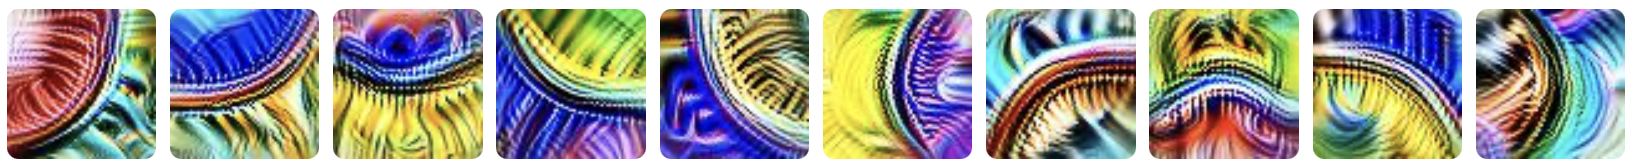
\includegraphics[width=1\linewidth]{images/curve_detector_3b379.png}
        \caption{}
        \label{fig:Ng1} 
    \end{subfigure}
    \medskip
    \begin{subfigure}[b]{0.75\textwidth}
        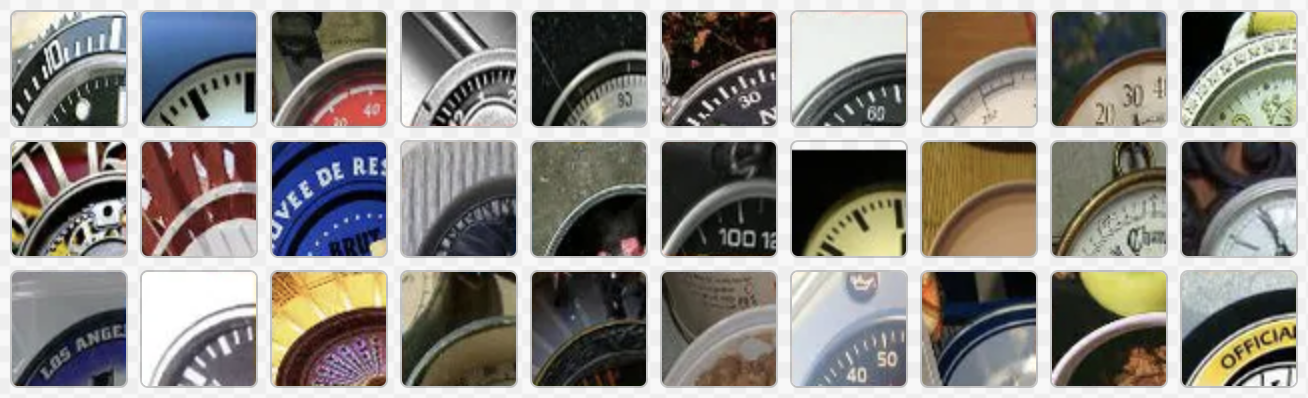
\includegraphics[width=1\linewidth]{images/dataset_samples.png}
        \caption{}
        \label{fig:Ng2}
    \end{subfigure}
    \caption{Wizualizacja neuronów zidentyfikowanych jako detektory krzywizn (a) oraz przykładowe obrazy ze zbioru danych (b) aktywujące te neurony w sieci \textit{InceptionV1}. Źródło: \cite{cammarata_2020_curve_detectors}, materiał udostępniony na licencji CC-BY 4.0.}
    \label{fig:curve_detector}
\end{figure}
\newline
Poza samą identyfikacją i weryfikacją selektywności neuronu, artykuł \textit{Zoom In} pokazuje również, w jaki sposób detektor ten jest zbudowany: analizując wagi łączące go z rodziną wcześniejszych detektorów linii o różnych orientacjach w poprzedniej warstwie, autorzy odczytują wprost z sieci algorytm detekcji krzywizny -- neuron sumuje pobudzenia od linii zorientowanych zgodnie z daną krzywizną i jednocześnie tłumi pobudzenia od linii o przeciwnej orientacji. \newline
\begin{figure}[h]
    \centering
    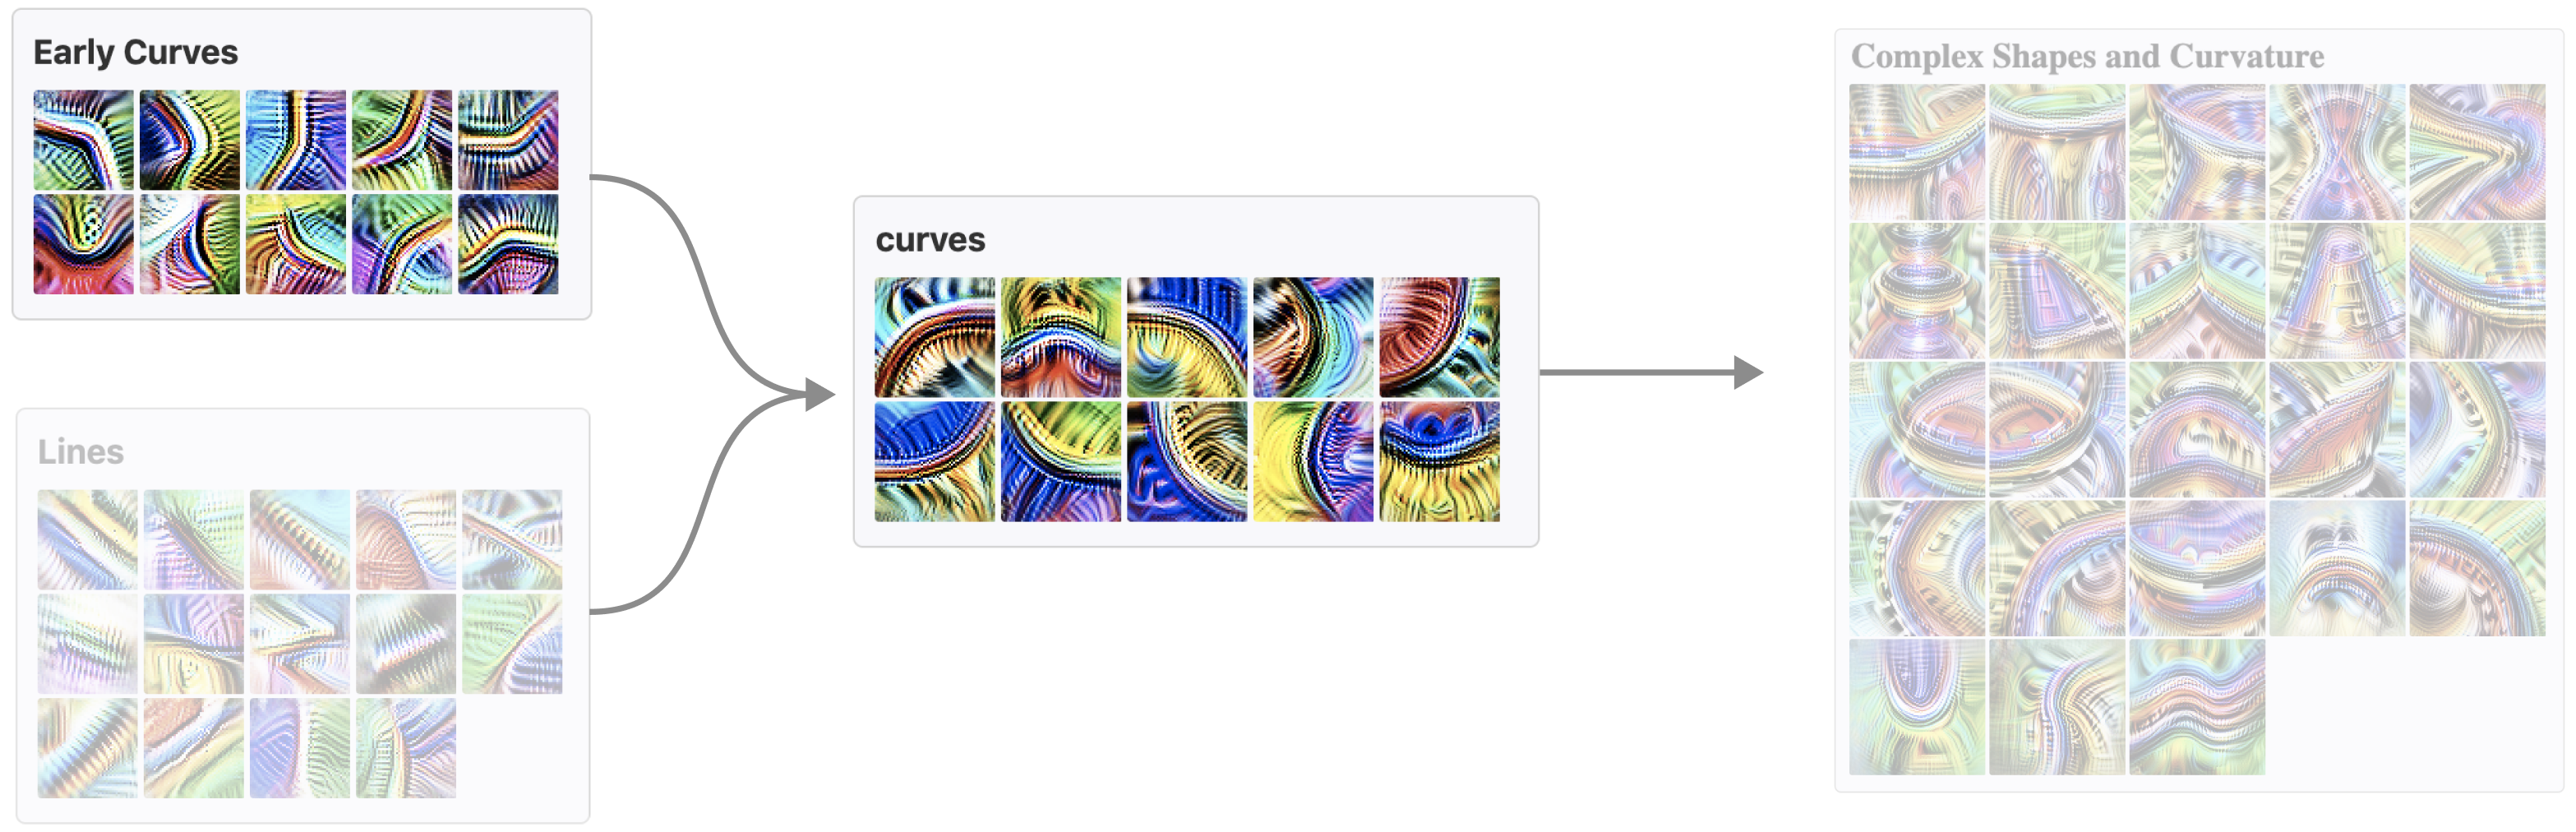
\includegraphics[width=1\textwidth]{images/curve_detector_circuit.png}
    \caption{Diagram wag ilustrujący obwód budujący detektory krzywizn z ważonej kombinacji wcześniejszych detektorów linii o różnych orientacjach. Źródło: \cite{olah_2020_zoom_in_circuits}, materiał udostępniony na licencji CC-BY 4.0.}
    \label{fig:curve_circuit_diagram}
\end{figure}
\newline
%Wizualizacja wag jako alternatywa dla analizy aktywacji - Visualizing Weights (Voss i in., 2021) -> kontekstualizacja, expanded weights, faktoryzacja (NMF) -> bezpośrednie powiązanie z planowaną analizą macierzy wag MLP (rozdz. 4) \newline -- obecnie poza zakresem pracy
Wszystkie omówione w tym podrozdziale prace -- od \textit{Feature Visualization}, przez \textit{Building Blocks of Interpretability} i \textit{Zoom In}, po \textit{Curve Detectors} oraz \textit{Visualizing Weights} -- łączy jedno istotne ograniczenie: cały program badawczy circuits rozwijany był niemal wyłącznie na sieciach konwolucyjnych przetwarzających obraz, a w większości przypadków na jednym, konkretnym, w pełni prześwietlonym modelu -- \textit{InceptionV1}. Podstawowe jednostki analizy -- krawędzie, linie, krzywizny, tekstury -- są więc z natury wizualne, a badane \enquote{fakty o świecie} sprowadzają się w praktyce do niskopoziomowych cech geometrycznych obrazu, nie do wiedzy faktograficznej czy relacji semantycznych, które stanowią przedmiot niniejszej pracy. Transfer tego programu badawczego na grunt architektury transformer i modeli językowych nie był przy tym automatyczny -- wymagał sformułowania nowego aparatu pojęciowego, dostosowanego do specyfiki strumienia rezydualnego, mechanizmu uwagi oraz warstw MLP pełniących funkcję pamięci klucz-wartość \cite{geva_2021_transformer_feedforward_key_value_memories}. Kontynuacją tego kierunku, prowadzoną w dużej mierze przez tych samych badaczy już w strukturach nowo powstałego \textit{Anthropic}, jest \textit{A Mathematical Framework for Transformer Circuits} \cite{elhage_2021_mathematical_framework_transformer_circuits}, formalizujący pojęcia obwodu i strumienia rezydualnego w kontekście transformerów -- oraz, opisany w dalszej części niniejszego rozdziału, problem superpozycji, wynikający bezpośrednio z napięcia zasygnalizowanego już w \textit{Zoom In}. Sposób, w jaki idee wypracowane na gruncie wizji komputerowej -- lokalizacja pojedynczej, dobrze scharakteryzowanej jednostki obliczeniowej oraz rekonstrukcja łączących je obwodów -- dają się przenieść na grunt wiedzy faktograficznej reprezentowanej przez modele językowe, jest tematem dalszego podrozdziału \ref{sec:interpretowalnosc_modeli_jezykowych}. \newline


\section{Architektura transformer}
\label{sec:architektura_transformer}
%TODO: może warto wyjaśnić czym jest atencja i wrzucić jakiś prosty matematyczny wzór albo schemat pokazujący jak działa (co jest mnożone przez co)
Architektura transformer, będąca dziś fundamentem niemal wszystkich dużych modeli językowych, została wprowadzona w pracy \textit{Attention Is All You Need} \cite{vaswani_2017_attention_is_all_you_need}, pierwotnie jako rozwiązanie zadania tłumaczenia maszynowego oparte na strukturze enkoder-dekoder. Podstawowym elementem tej architektury jest blok transformera, złożony z dwóch podwarstw. Ponieważ mechanizm uwagi sam w sobie jest niewrażliwy na kolejność tokenów w sekwencji, wejściowe osadzenia (ang. \textit{embedding}) tokenów są najpierw wzbogacane o kodowanie pozycyjne (w oryginalnej pracy -- sinusoidalne), niosące informację o miejscu tokenu w sekwencji. Pierwszą podwarstwą jest wielogłowy mechanizm samo-uwagi (ang. \textit{multi-head self-attention}), pozwalający każdej pozycji w sekwencji ważyć i agregować informacje pochodzące z pozostałych pozycji, przy czym równoległe działanie wielu głów uwagi umożliwia jednoczesne wychwytywanie różnych typów zależności między tokenami. Drugą podwarstwą jest warstwa feed-forward (MLP) -- dwie transformacje liniowe rozdzielone nieliniowością, stosowane niezależnie i identycznie do każdej pozycji z osobna. Obie podwarstwy opatrzone są połączeniami rezydualnymi, których koncepcja została zapożyczona z wcześniejszych prac nad głębokimi sieciami konwolucyjnymi \cite{he_2015_deep_residual_learning}, oraz normalizacją warstwową \cite{ba_2016_layer_normalization}, stabilizującą trening bardzo głębokich stosów takich bloków. Ten schemat, powielony wielokrotnie w głąb sieci, stanowi wspólny szkielet terminologiczny dla całej dalszej części niniejszego rozdziału. Schemat architektury przedstawiony został na rysunku \ref{fig:transofrmer_architecture}. \newline
\begin{figure}[h]
    \centering
    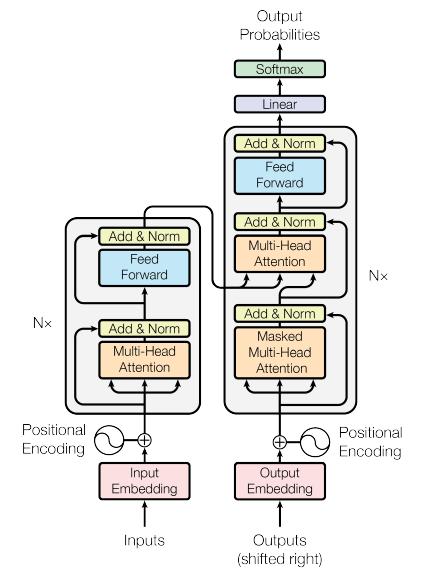
\includegraphics[width=0.5\textwidth]{images/transformer_architecture.png}
    \caption{Architektura modelu transformera zaprezentowana w pracy \textit{Attention Is All You Need} \cite{vaswani_2017_attention_is_all_you_need}. Przedstawia opisane wyżej podwarstwy mechanizmu uwagi oraz MLP wraz z połączeniami rezydualnymi połączone w bloki.}
    \label{fig:transofrmer_architecture}
\end{figure} % TODO: rozpikselizowany obraz
\newline
Choć sama architektura opisana przez Vaswaniego i in. wprowadza połączenia rezydualne jako techniczny środek ułatwiający propagację gradientu w głębokich sieciach, dopiero praca \textit{A Mathematical Framework for Transformer Circuits} \cite{elhage_2021_mathematical_framework_transformer_circuits} (omówiona szerzej w podrozdziale \ref{sec:interpretowalnosc_modeli_jezykowych}) opisuje ten mechanizm w kategorii możliwego do interpretowania, wprowadzając pojęcie strumienia rezydualnego (ang. \textit{residual stream}). Zgodnie z tym ujęciem, połączenia rezydualne można traktować jako wspólną \enquote{magistralę} informacyjną, przebiegającą przez cały model -- każda kolejna podwarstwa, zarówno attention, jak i MLP, odczytuje z niej swój stan wejściowy, wykonuje właściwe obliczenie, po czym addytywnie dopisuje wynik z powrotem do strumienia, nigdy go nie nadpisując. W konsekwencji stan strumienia w danej pozycji sekwencji jest sumą wkładów wszystkich poprzedzających go warstw, a każda kolejna warstwa ma pełny dostęp do wszystkiego, co zostało zapisane wcześniej. Istotnym ograniczeniem tego mechanizmu jest jednak niska, stała wymiarowość samego strumienia względem potencjalnie znacznie większej liczby komponentów, które chciałyby z niego korzystać jednocześnie -- warstwy muszą więc konkurować o ograniczoną przestrzeń kierunków, w których mogą zapisywać swoje wyniki. Ten problem strukturalnego \enquote{wąskiego gardła} stanowi bezpośredni punkt wyjścia do omawianego w dalszej części rozdziału zjawiska superpozycji. \newline
O ile poprzedni akapit opisuje strumień rezydualny jako wspólną magistralę, o tyle mechanizm uwagi i warstwa MLP pełnią w niej odmienne funkcje. Głowy uwagi przenoszą informację między pozycjami w sekwencji -- pozwalają danej pozycji \enquote{spojrzeć} na inne tokeny i skopiować lub zagregować niesione przez nie informacje z powrotem do strumienia rezydualnego we własnej pozycji. MLP natomiast operuje wyłącznie lokalnie, przetwarzając zawartość strumienia w obrębie pojedynczej pozycji, bez dostępu do pozostałych tokenów sekwencji. Najpełniej zinżynierowanym przykładem obwodu zbudowanego z tego pierwszego mechanizmu są tzw. \textit{induction heads}, opisane w pracy \textit{In-context Learning and Induction Heads} \cite{olsson_2022_induction_heads}. Autorzy identyfikują parę współpracujących głów uwagi rozłożonych w różnych warstwach modelu: głowę poprzedniego tokenu (ang. \textit{previous-token head}), zapisującą do strumienia rezydualnego informację o tokenie poprzedzającym daną pozycję, oraz właściwą głowę indukcyjną, która -- korzystając z tego zapisu za pośrednictwem tej samej magistrali strumienia rezydualnego -- przeszukuje wcześniejszy kontekst w poszukiwaniu poprzedniego wystąpienia bieżącego tokenu i kopiuje token, który wówczas po nim nastąpił, realizując w ten sposób prosty wzorzec dopasowania sekwencji [A][B]...[A]$\rightarrow$[B]. Jest to bezpośredni analog detektora krzywizny omówionego w podrozdziale \ref{sec:podejscie_obwodowe} -- pojedynczy obwód, osadzony w architekturze transformera i operujący na tokenach języka zamiast na pikselach obrazu, stanowiący pierwszy dowód na to, że program badawczy circuits daje się skutecznie przenieść z sieci wizyjnych na modele językowe. 
% MLP, w przeciwieństwie do tego mechanizmu opartego na przenoszeniu informacji, jest naturalnym kandydatem na miejsce jej przechowywania -- hipoteza ta, wraz z uzasadniającą ją interpretacją warstw MLP jako pamięci klucz-wartość, zostanie szerzej omówiona w podrozdziale \ref{sec:lokalizacja_wiedzy}. 
\newline
Oryginalna architektura opisana przez Vaswaniego i in. została zaprojektowana jako model enkoder-dekoder, w którym enkoder przetwarza całą sekwencję wejściową jednocześnie, a dekoder -- korzystając dodatkowo z mechanizmu \textit{cross-attention} czerpiącego z wyjścia enkodera -- generuje sekwencję wyjściową token po tokenie. Modele językowe typu GPT (ang. \textit{decoder-only}), zapoczątkowane pracą \textit{Improving Language Understanding by Generative Pre-Training} \cite{radford_2018_improving_language_understanding} i rozwinięte w \textit{Language Models are Unsupervised Multitask Learners} \cite{radford_2019_language_models_unsupervised_multitask_learners}, upraszczają ten schemat, odrzucając enkoder oraz cross-attention i pozostawiając wyłącznie stos bloków dekodera. Kluczową modyfikacją jest przy tym zastosowanie zamaskowanego (przyczynowego, ang. \textit{causal}) self-attention -- każda pozycja w sekwencji może uwzględniać w obliczeniu uwagi wyłącznie tokeny ją poprzedzające, nigdy przyszłe. Ograniczenie to sprawia, że model można trenować i wykorzystywać w sposób autoregresywny: przewidując kolejny token wyłącznie na podstawie tokenów dotychczas wygenerowanych. O ile praca Radforda i in. z 2018 roku traktuje generatywny pretrening przede wszystkim jako etap wstępny poprzedzający dostrajanie pod konkretne zadanie, o tyle \textit{GPT-2} \cite{radford_2019_language_models_unsupervised_multitask_learners} pokazuje, że sam czysty pretrening języka naturalnego, bez żadnego dostrajania zadaniowego, prowadzi do modelu zdolnego generalizować do wielu zadań jednocześnie -- ugruntowując tym samym architekturę dekoderową jako samodzielny, dominujący dziś paradygmat budowy modeli językowych. To właśnie ten wariant architektoniczny wybrano jako podstawę eksperymentów niniejszej pracy, zgodnie z założeniami przedstawionymi w podrozdziale \ref{sec:cele}. \newline

\section{Interpretowalność modeli językowych}
\label{sec:interpretowalnosc_modeli_jezykowych}
Podrozdział \ref{sec:architektura_transformer} przedstawił architekturę transformer w ujęciu czysto strukturalnym -- jako następujące po sobie bloki uwagi i MLP, komunikujące się za pośrednictwem strumienia rezydualnego. Sam ten opis nie rozstrzyga jednak, w jaki sposób można zbadać, co dzieje się wewnątrz tak zdefiniowanej struktury podczas przetwarzania konkretnego tekstu. Pytanie to, postawione ogólnie w podrozdziale \ref{sec:interpretowalnosc_sieci_neuronowych}, powraca tutaj w wersji dostosowanej do modeli językowych, wzdłuż tego samego podziału na podejście reprezentacyjne i mechanistyczne. Pierwsze z nich pyta, jaka informacja jest w danym momencie zakodowana w strumieniu rezydualnym -- realizują je metody sondujące (podrozdział \ref{sec:probing}) oraz logit lens (podrozdział \ref{sec:logit_lens}), operujące wyłącznie na aktywacjach modelu. Drugie, zgodnie z duchem podejścia obwodowego z podrozdziału \ref{sec:podejscie_obwodowe}, pyta wprost, jaki mechanizm zapisany w wagach modelu tę informację wytwarza -- odpowiada na to matematyczny opis obwodów transformera (podrozdział \ref{sec:framework_obwodow}), rozwijający program \textit{circuits} na grunt architektury opisanej w poprzednim podrozdziale. Obie tradycje dostarczają narzędzi wykorzystanych w dalszej części pracy, w tym w potoku analitycznym opisanym w rozdziale 3. \newline
\subsection{Metody sondujące (ang. \textit{probing classifiers})}
\label{sec:probing}
Najprostszym sposobem zadania pytania, jaka informacja o przetwarzanym tekście jest zakodowana w reprezentacji danej warstwy, jest pominięcie mechanizmu jej powstawania i sprawdzenie jedynie, czy informacja ta daje się z tej reprezentacji odczytać. Metodę tę, nazywaną sondowaniem (ang. \textit{probing}), sformalizowali Guillaume Alain i Yoshua Bengio \cite{alain_2016_understanding_intermediate_layers_using_linear_classifier_probes}: polega ona na zamrożeniu wag badanej sieci i wytrenowaniu dodatkowego, zwykle liniowego klasyfikatora (tzw. sondy, ang. \textit{probe}) na aktywacjach wybranej warstwy, mającego przewidzieć z góry zdefiniowaną własność przetwarzanych danych. Wysoka skuteczność takiej sondy świadczy o tym, że badana własność jest w danej warstwie reprezentowana w sposób liniowo dekodowalny -- niezależnie od tego, jaki mechanizm doprowadził do jej zakodowania. \newline
Metodę tę zastosowali do modeli językowych Ian Tenney i współpracownicy w pracy \textit{BERT Rediscovers the Classical NLP Pipeline} \cite{tenney_2019_bert_rediscovers_classical_nlp_pipeline}, trenując sondy do klasycznych zadań lingwistycznych -- znakowania części mowy, analizy składniowej, przypisywania ról semantycznych oraz rozwiązywania koreferencji -- na zamrożonych reprezentacjach kolejnych warstw modelu BERT. Autorzy pokazali, że zadania te dają się uporządkować zgodnie z rosnącą głębokością sieci w kolejności odpowiadającej klasycznemu potokowi przetwarzania języka naturalnego -- zadania powierzchniowe są najlepiej dekodowalne z warstw wcześniejszych, a zadania wymagające przetwarzania bardziej abstrakcyjnego z warstw głębszych. Wynik ten stanowi językowy odpowiednik hierarchii cech zaobserwowanej wcześniej w sieciach konwolucyjnych (podrozdział \ref{sec:wczesne_prace_wizualizacja}) -- od krawędzi po całe obiekty -- i dostarczył jednego z pierwszych empirycznych dowodów na to, że głębokość sieci językowej koreluje z poziomem abstrakcji przetwarzanej informacji. \newline
Warto przy tym zaznaczyć, że wyniki Tenney i współpracowników uzyskano na modelu BERT, a więc architekturze enkoderowej, przetwarzającej sekwencję dwukierunkowo. Sama metoda sondująca jest jednak niezależna od architektury i w tej samej postaci daje się zastosować do modeli dekoderowych, takich jak model wykorzystany w niniejszej pracy (podrozdział \ref{sec:cele}).
\subsection{Logit lens}
\label{sec:logit_lens}
W odróżnieniu od metod sondujących, wymagających wytrenowania dodatkowego klasyfikatora na aktywacjach badanej warstwy, modele dekoderowe typu GPT dają możliwość odczytania stanu pośredniego strumienia rezydualnego bez żadnego dodatkowego treningu. Wynika to z samej konstrukcji tych modeli: ostateczny stan strumienia rezydualnego jest, po zastosowaniu normalizacji warstwowej (ang. \textit{layer normalization}), rzutowany na przestrzeń słownika za pomocą macierzy unembeddingu, dającej w wyniku rozkład prawdopodobieństwa nad kolejnym tokenem. Technika logit lens, powstała w formie nieformalnego wpisu na forum \textit{LessWrong} \cite{nostalgebraist_2020_logit_lens}, wykorzystuje ten sam mechanizm przedwcześnie -- rzutuje na przestrzeń słownika stan strumienia rezydualnego odczytany z warstwy pośredniej, tak jakby był on już stanem końcowym. Powtarzając tę operację dla kolejnych warstw modelu, można prześledzić, jak rozkład przewidywanego tokenu ewoluuje wraz z głębokością sieci -- od niespecyficznych, często wysokoczęstotliwościowych przewidywań we wczesnych warstwach, po coraz bardziej trafną i ostateczną predykcję w warstwach końcowych. \newline
Metoda ta przyjęła się jako standardowe narzędzie eksploracyjne w badaniach nad interpretowalnością modeli językowych, ze względu na jej prostotę i brak kosztu obliczeniowego związanego z treningiem. Warto przy tym zaznaczyć, że technika ta niejawnie zakłada, iż reprezentacje pośrednie warstw są wyrażone w tej samej bazie co reprezentacja warstwy końcowej. Założenie to jest jednak jedynie przybliżeniem, przez co zwłaszcza w warstwach początkowych rzutowane rozkłady bywają niespójne i trudne do zinterpretowania jako sensowne predykcje kolejnego tokenu. Im głębsza jednak warstwa, z której pochodzi rzutowany stan, tym rzutowana predykcja staje się zwykle coraz bardziej spójna i zbliżona do finalnego wyniku modelu.

\subsection{Matematyczny opis obwodów transformera}
\label{sec:framework_obwodow}
%TODO: czy nie trzeba sprecyzować czemu ta metoda jest opisywana obok probing i logit lens? Tutaj chyba słabe jest to wytłumaczenie
O ile metody sondujące i logit lens analizują stan strumienia rezydualnego wywołany przez konkretny tekst wejściowy, o tyle praca \textit{A Mathematical Framework for Transformer Circuits} \cite{elhage_2021_mathematical_framework_transformer_circuits} proponuje podejście działające wyłącznie na poziomie wag modelu. Punktem wyjścia jest obserwacja, że skoro każda podwarstwa komunikuje się ze strumieniem rezydualnym (podrozdział \ref{sec:architektura_transformer}) wyłącznie za pośrednictwem operacji liniowych, to nawet odległe od siebie warstwy można opisać efektywną zależnością liniową, wyliczoną wprost z iloczynu ich macierzy wag -- bez uruchamiania modelu na jakichkolwiek danych. Na tej podstawie autorzy rozkładają mechanizm uwagi na dwa niezależne obwody: decydujący o tym, które pozycje w sekwencji są brane pod uwagę, oraz decydujący, jaka informacja zostaje na tej podstawie skopiowana z powrotem do strumienia. Takie podejście pozwoliło formalnie wyjaśnić działanie induction heads, opisanych w podrozdziale \ref{sec:architektura_transformer} \cite{olsson_2022_induction_heads}, jako przykład współpracy dwóch głów uwagi rozłożonych w różnych warstwach. \newline
Analiza ta prowadzi jednak autorów do istotnego zastrzeżenia wobec własnej metody: ze względu na liniową, addytywną strukturę strumienia rezydualnego, nie posiada on żadnej wyróżnionej, \enquote{uprzywilejowanej bazy} (ang. \textit{privileged basis}) -- nic nie gwarantuje, że pojedynczy neuron czy pojedynczy wymiar strumienia odpowiada jednemu, czytelnemu konceptowi. Co więcej, liczba komponentów obliczeniowych (neuronów warstw MLP, wymiarów wyniku głów uwagi) konkurujących o miejsce w strumieniu znacząco przewyższa jego wymiarowość, zmuszając je -- jak to określają sami autorzy -- do komunikowania się w superpozycji. Zjawisko to, jedynie zasygnalizowane w opisywanej pracy, stanowi przedmiot kolejnego podrozdziału.

\section{Problem superpozycji i geneza rzadkich autoenkoderów}
\label{sec:superpozycja}
Podrozdział \ref{sec:framework_obwodow} zasygnalizował zjawisko superpozycji, nie wyjaśniając jednak wprost, na czym ono polega -- ograniczona, stała wymiarowość strumienia rezydualnego, zestawiona z brakiem jego uprzywilejowanej bazy, zmusza konkurujące o miejsce w nim komponenty obliczeniowe do dzielenia się tymi samymi kierunkami. Niniejszy podrozdział wyjaśnia mechanikę tego zjawiska na przykładzie modelu roboczego zaproponowanego przez zespół Anthropic, po czym omawia jego konsekwencje dla interpretacji pojedynczych jednostek sieci (podrozdział \ref{sec:polisemantycznosc}) oraz sposób, w jaki próba jego odwrócenia doprowadziła do sformułowania hipotezy słownikowej -- bezpośredniego pomostu do rzadkich autoenkoderów, będących przedmiotem dalszej części niniejszego rozdziału (podrozdział \ref{sec:hipoteza_slownikowa}).
\subsection{Zjawisko superpozycji}
\label{sec:zjawisko_superpozycji}
Punktem wyjścia dla zrozumienia superpozycji jest tzw. hipoteza reprezentacji liniowej (ang. \textit{linear representation hypothesis}), zgodnie z którą pojedyncza cecha (ang. \textit{feature}) -- rozumiana jako odrębny, interpretowalny koncept reprezentowany przez sieć -- odpowiada nie pojedynczemu neuronowi, lecz pewnemu kierunkowi w wielowymiarowej przestrzeni aktywacji. Założenie to obecne już w metodach sondujących i w programie circuits omówionych we wcześniejszych podrozdziałach, prowadzi do pytania, ile takich kierunków sieć jest w stanie jednocześnie utrzymać, skoro liczba potencjalnie istotnych konceptów świata rzeczywistego, które model powinien rozróżniać, znacząco przewyższa liczbę neuronów dostępnych w pojedynczej warstwie. \newline
Odpowiedzi na to pytanie udzielają Nelson Elhage i współpracownicy z Anthropic w pracy \textit{Toy Models of Superposition} \cite{elhage_2022_toy_models_of_superposition}, konstruując silnie uproszczony model, w którym zjawisko to można badać w pełni kontrolowanych warunkach: wektor cech o wymiarowości znacząco przewyższającej wymiarowość warstwy ukrytej jest do niej liniowo rzutowany, a następnie odtwarzany z powrotem za pomocą tej samej macierzy wag i nieliniowości ReLU. Każda cecha wejściowa charakteryzuje się rzadkością (ang. \textit{sparsity}) -- prawdopodobieństwem, że w danej chwili przyjmuje wartość zerową -- oraz ważnością (ang. \textit{importance}), określającą, jak silnie błąd jej rekonstrukcji obciąża łączną funkcję straty. \newline
Autorzy pokazują, że zachowanie modelu silnie zależy od rzadkości reprezentowanych cech. Gdy cechy są gęste, a przestrzeń ukryta nie wystarcza do zakodowania wszystkich z nich, model reprezentuje jedynie tyle cech, ile ma do dyspozycji wymiarów, pomijając resztę. W miarę wzrostu rzadkości model zaczyna jednak reprezentować więcej cech niż posiada wymiarów, przypisując im nieortogonalne, nakładające się na siebie kierunki -- godząc się na pewną wzajemną interferencję między nimi w zamian za zwiększoną pojemność reprezentacyjną. Właśnie to zjawisko autorzy nazywają superpozycją, a umożliwia je zastosowana w kroku rekonstrukcji nieliniowość ReLU, tłumiąca drobną interferencję pochodzącą od nieaktywnych w danej chwili cech. \newline
Zjawisko to ma bezpośrednie konsekwencje dla sposobu, w jaki należy interpretować pojedyncze jednostki sieci -- zagadnieniu temu poświęcony jest kolejny podrozdział.
\subsection{Polisemantyczność}
\label{sec:polisemantycznosc}
Zjawisko superpozycji opisane w poprzednim podrozdziale dostarcza mechanistycznego wyjaśnienia obserwacji poczynionej już w podrozdziale \ref{sec:podejscie_obwodowe} -- autorzy \textit{Zoom In} \cite{olah_2020_zoom_in_circuits} zauważyli, że część neuronów sieci \textit{InceptionV1} jest polisemantyczna, tzn. aktywuje się w odpowiedzi na kilka odrębnych, niepowiązanych ze sobą pojęć jednocześnie \cite{olah_2020_zoom_in_circuits}. Pracy \textit{Toy Models of Superposition} dokładniej skupia się na tym zjawisku: skoro sieć reprezentuje więcej cech niż posiada wymiarów, przypisując im nieortogonalne, nakładające się kierunki, to pojedynczy neuron z konieczności bierze udział w kodowaniu wielu z nich naraz. Polisemantyczność jest więc oczekiwaną konsekwencją superpozycji przy ograniczonej wymiarowości sieci. \newline
Wniosek ten podważa założenie leżące u podstaw większości metod omówionych w podrozdziałach \ref{sec:wczesne_prace_wizualizacja} i \ref{sec:podejscie_obwodowe} -- że pojedyncza, dobrze scharakteryzowana jednostka sieci (neuron, kanał) stanowi naturalną, monosemantyczną jednostkę analizy. Zarówno maksymalizacja aktywacji \cite{olah_2017_feature_visualization}, jak i studium przypadku pojedynczego neuronu w \textit{Curve Detectors} \cite{cammarata_2020_curve_detectors} zakładają, że wyjaśnienie znaczenia jednego neuronu jest zadaniem dobrze postawionym. W obecności superpozycji założenie to jest jednak spełnione jedynie częściowo -- część neuronów faktycznie odpowiada w przybliżeniu jednemu konceptowi, inne zaś są superpozycją wielu niepowiązanych ze sobą cech, co czyni ich bezpośrednią interpretację niejednoznaczną. \newline
Powyższe ograniczenie rodzi pytanie, czy możliwe jest odzyskanie z superpozycji jednostek bliższych rzeczywistym, monosemantycznym cechom, zamiast poprzestawać na analizie pojedynczych, potencjalnie polisemantycznych neuronów. Remedium na ten problem, wywodzące się z tzw. hipotezy słownikowej, jest omówione w kolejnym podrozdziale.
\subsection{Hipoteza słownikowa}
\label{sec:hipoteza_slownikowa}
Skoro, jak pokazano w podrozdziale \ref{sec:zjawisko_superpozycji}, sieć koduje rzadkie cechy jako nadpełny (ang. \textit{overcomplete}), nakładający się na siebie zestaw kierunków w przestrzeni aktywacji, to zadanie odzyskania tych cech można sformułować jako problem odwrotny: obserwowany wektor aktywacji jest rzadką kombinacją liniową nieznanych, rzeczywistych kierunków bazowych, a celem jest odtworzenie zarówno tych kierunków, jak i rzadkich współczynników, z jakich każda konkretna aktywacja jest złożona. Sformułowany w ten sposób problem odpowiada dokładnie klasycznemu zagadnieniu rzadkiego uczenia się słownika (ang. \textit{sparse dictionary learning}), znanego wcześniej z zastosowań poza dziedziną modeli językowych. \newline
Zastosowanie tego podejścia do aktywacji sieci neuronowych zaproponowali Lee Sharkey, Dan Braun i Beren Millidge w raporcie badawczym \textit{Taking Features Out of Superposition With Sparse Autoencoders} \cite{sharkey_2022_taking_features_out_of_superposition}, bezpośrednio nawiązującym do wyników opisanych w \textit{Toy Models of Superposition}. Autorzy proponują wytrenowanie rzadkiego autoenkodera (ang. \textit{Sparse Autoencoder}, SAE) -- sieci złożonej z enkodera rzutującego aktywacje badanego modelu w znacznie szerszą, nadpełną przestrzeń ukrytą, oraz dekodera odtwarzającego z niej oryginalną aktywację jako jej liniową kombinację. Kara za brak rzadkości, nałożona na aktywacje warstwy ukrytej, wymusza, by w rekonstrukcji każdej pojedynczej aktywacji brała udział jedynie niewielka liczba kierunków tego nadpełnego słownika -- w zamierzeniu odpowiadających pojedynczym, monosemantycznym cechom, zamiast ich superpozycji. \newline
Propozycja ta, sformułowana jeszcze jako wstępny raport badawczy i zweryfikowana wyłącznie na niewielkich modelach, otworzyła jednak drogę do serii prac stosujących rzadkie autoenkodery bezpośrednio do modeli językowych -- ich przegląd jest przedmiotem kolejnego podrozdziału.

\section{Rzadkie autoenkodery (SAE) jako narzędzie dekompozycji reprezentacji}
\label{sec:sae_dekompozycja}
Hipoteza słownikowa omówiona w poprzednim podrozdziale (\ref{sec:hipoteza_slownikowa}) wprowadzała koncepcję rzadkiego autoenkodera zweryfikowaną na modelu roboczym -- pojedynczym, jednowarstwowym transformerze, dobranym tak, by ułatwić kontrolowaną analizę. Otwarte pozostawało więc pytanie, czy metoda ta przenosi się na modele o istotnie większej skali oraz czy wyodrębnione w ten sposób kierunki rzeczywiście odpowiadają czytelnym, monosemantycznym konceptom. Niniejszy podrozdział prześledzi, jak na te pytania odpowiedziała kolejna fala prac -- począwszy od pierwszej walidacji podejścia na realnych modelach językowych, przez rozwinięcia architektoniczne, aż po metodykę przyjętą w niniejszej pracy.

\subsection{Pierwsze zastosowania SAE na aktywacjach modeli językowych}
\label{sec:sae_pierwsze_prace}
Jesienią 2023 roku, niezależnie od siebie i w odstępie zaledwie kilku tygodni, opublikowane zostały dwie prace \cite{cunningham_2023_sparse_autoencoders_highly_interpretable_features, bricken_2023_towards_monosemanticity_dictionary_learning}, które po raz pierwszy zastosowały rzadkie autoenkodery do aktywacji rzeczywistych modeli językowych. Dwa niezależne zespoły, stosując odmienne modele i protokoły ewaluacji, doszły do zgodnego wniosku, że rzadkie autoenkodery rzeczywiście dekomponują aktywacje na kierunki bardziej interpretowalne niż kierunki wskazywane przez metody alternatywne. \newline
Hoagy Cunningham i współpracownicy w pracy \textit{Sparse Autoencoders Find Highly Interpretable Features in Language Models} \cite{cunningham_2023_sparse_autoencoders_highly_interpretable_features} skupili się przede wszystkim na ilościowym udowodnieniu tej przewagi. Wyodrębnione przez SAE kierunki porównali z kierunkami wskazywanymi przez metody bazowe -- analizę głównych składowych (ang. \textit{Principal Component Analysis}, PCA), analizę składowych niezależnych (ang. \textit{Independent Component Analysis}, ICA) oraz surowe kierunki odpowiadające pojedynczym neuronom. Do oceny interpretowalności każdego kierunku zastosowali zautomatyzowaną metodę, wywodzącą się z wcześniejszych prac nad wyjaśnianiem pojedynczych neuronów: dla danej cechy generowany jest opis słowny na podstawie fragmentów tekstu najsilniej ją aktywujących, a jakość tego opisu weryfikuje się, sprawdzając, na ile pozwala on przewidzieć aktywację cechy na nowym, niewidzianym wcześniej fragmencie tekstu. Zgodnie z tą metryką kierunki wskazywane przez SAE okazały się systematycznie bardziej interpretowalne niż kierunki wskazywane przez każdą z metod bazowych.
\begin{figure}[h]
    \centering
    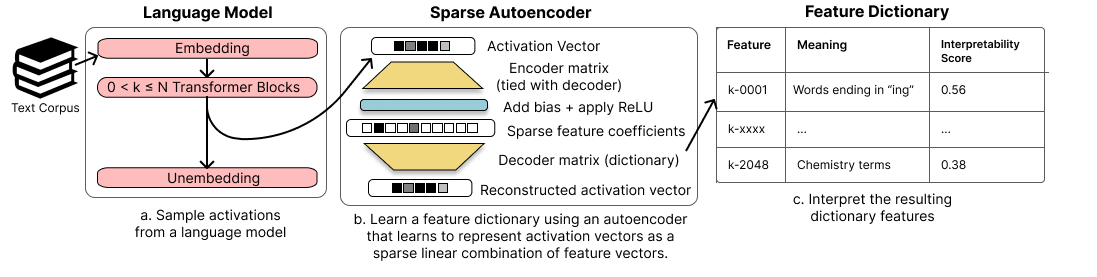
\includegraphics[width=\textwidth]{images/sae_training.png}
    \caption{Ogólny proces uczenia modelu autoenkodera stosowany w większości eksperymentów, a także zastosowany na potrzeby niniejszej pracy. Grafika pochodzi z pracy \textit{Sparse Autoencoders Find Highly Interpretable Features in Language Models} \cite{cunningham_2023_sparse_autoencoders_highly_interpretable_features}.}
    \label{fig:sae_training}
\end{figure}
\newline
Równolegle Trenton Bricken i współpracownicy z Anthropic opublikowali \textit{Towards Monosemanticity: Decomposing Language Models With Dictionary Learning} \cite{bricken_2023_towards_monosemanticity_dictionary_learning} -- pracę skupioną w mniejszym stopniu na porównaniu z metodami alternatywnymi, a w większym na dogłębnej analizie samego procesu treningu SAE i wypracowaniu metodyki jego oceny, która stała się później de facto standardem przyjmowanym przez kolejne prace omówione w dalszej części niniejszego rozdziału. Eksperymenty przeprowadzono na celowo bardzo małym modelu -- jednowarstwowym transformerze z warstwą MLP liczącą 512 neuronów -- co pozwoliło na wielokrotne powtórzenie treningu przy różnych wartościach hiperparametrów i rozmiarach słownika cech. Autorzy zdefiniowali dwie podstawowe, wzajemnie sprzeczne miary jakości dekompozycji: stratę rekonstrukcji (ang. \textit{reconstruction loss}), mierzącą, jak wiernie autoenkoder odtwarza oryginalną aktywację, oraz rzadkość $L0$, rozumianą jako średnią liczbę jednocześnie aktywnych cech przypadającą na pojedynczą aktywację wejściową. Zmniejszanie $L0$ zwykle pogarsza rekonstrukcję, co czyni dobór właściwego punktu na tym kompromisie centralnym zagadnieniem praktycznym przy treningu. \newline
Praca ta zidentyfikowała również dwa zjawiska, które muszą być brane pod uwagę przy każdym treningu SAE. Pierwszym są martwe cechy (ang. \textit{dead features}) -- kierunki słownika, które w trakcie treningu przestają się aktywować dla jakiegokolwiek fragmentu danych i nigdy nie powracają do użycia, efektywnie zmniejszając rzeczywistą pojemność autoenkodera poniżej nominalnego rozmiaru jego słownika. Drugim jest zjawisko rozszczepiania cech (ang. \textit{feature splitting}): w miarę zwiększania rozmiaru słownika pojedyncza, szeroka cecha wyodrębniona przy mniejszym słowniku rozszczepia się na kilka węższych, bardziej wyspecjalizowanych cech przy słowniku większym -- co sugeruje, że granice pomiędzy konceptami reprezentowanymi przez sieć nie są ustalone raz na zawsze, lecz zależą od rozdzielczości, z jaką próbujemy je odczytać.

\subsection{Sterowanie cechami (ang. \textit{feature steering})}
\label{sec:sae_feature_steering}
Metody omówione w poprzednim podrozdziale weryfikowały jakość dekompozycji SAE metrykami natury korelacyjnej -- zgodnością automatycznie wygenerowanego opisu cechy z tekstem ją aktywującym, stratą rekonstrukcji czy rzadkością $L0$. Żadna z nich nie odpowiada jednak wprost na pytanie, czy dana cecha rzeczywiście ma wpływ na zachowanie modelu, czy jedynie koreluje z pewnym wzorcem obecnym w danych wejściowych. Już Bricken i współpracownicy \cite{bricken_2023_towards_monosemanticity_dictionary_learning} zaproponowali prostą formę takiej weryfikacji: sztuczne wymuszenie ustalonej wartości aktywacji wybranej cechy podczas generowania tekstu (ang. \textit{feature steering}) i obserwację wynikającej z tego zmiany zachowania modelu. \newline
Templeton i współpracownicy \cite{templeton_scaling_monosemanticity} pokazali, że ta sama technika generalizuje się do modelu o skali produkcyjnej -- wzmacniając sztucznie aktywację pojedynczej cechy w modelu \textit{Claude 3 Sonnet}, uzyskali przewidywalną, spójną zmianę generowanego tekstu (najczęściej cytowanym przykładem jest cecha powiązana z mostem Golden Gate, której wymuszona aktywacja sprawiała, że model nawiązywał do mostu niezależnie od tematu rozmowy). Istotność tego wyniku nie leży jednak w samej anegdotyczności przykładu, lecz w tym, że stanowi on bezpośredni dowód na związek przyczynowy, między wyodrębnioną cechą a zachowaniem modelu -- odróżniając w ten sposób walidację SAE od walidacji metod atrybucyjnych opisanych w podrozdziale \ref{sec:wczesne_prace_wizualizacja}, które takiej przyczynowości wprost nie gwarantowały. Wzorzec ten -- lokalizacja cechy, a następnie jej przyczynowa weryfikacja poprzez interwencję -- zostanie wykorzystany również w metodyce walidacji przyjętej w niniejszej pracy. \newline
Mimo tych sukcesów, zarówno na małej, jak i produkcyjnej skali, sama architektura rzadkiego autoenkodera stosowana we wszystkich dotychczas omówionych pracach pozostawała niezmieniona od czasu \textit{Toy Models of Superposition} -- a wraz z nią nierozwiązany problem systematycznego zaniżania siły rekonstruowanych aktywacji, do którego odnosi się kolejny podrozdział.

\subsection{Warianty architektoniczne}
\label{sec:sae_warianty}
Wspólnym mianownikiem architektury SAE stosowanej we wszystkich dotychczas omówionych pracach był enkoder liniowy z nieliniowością ReLU, trenowany z karą $L1$ nałożoną na aktywacje warstwy ukrytej -- dokładnie taki, jaki zaproponowali Sharkey i współpracownicy w \cite{sharkey_2022_taking_features_out_of_superposition}. Kara $L1$, choć skuteczna w wymuszaniu rzadkości, wprowadza jednak systematyczne obciążenie zwane \textit{shrinkage}: ponieważ kara ta rośnie liniowo wraz z wielkością aktywacji niezależnie od tego, czy dana wielkość jest optymalna dla wiernej rekonstrukcji, optymalizacja premiuje zaniżanie aktywacji względem wartości, która najlepiej odtworzyłaby oryginalny sygnał. W efekcie nawet poprawnie zidentyfikowana, rzeczywiście aktywna cecha zostaje odtworzona z systematycznie zaniżoną siłą, co pogarsza jakość rekonstrukcji ponad to, czego wymagałaby sama rzadkość. \newline
Pierwszą próbą adresującą ten problem był \textit{Gated SAE}, zaproponowany przez Rajamanoharana i współpracowników \cite{rajamanoharan_2024a_gated_sparse_autoencoders}. Autorzy rozdzielili dwie decyzje, które w standardowym SAE podejmowane są łącznie przez tę samą nieliniowość: czy dana cecha powinna być aktywna, oraz jaką powinna mieć wielkość. Pierwszą decyzję podejmuje osobna gałąź bramkująca, karana za pomocą $L1$, drugą zaś -- gałąź odpowiedzialna wyłącznie za wielkość aktywacji, nieobjęta tą karą. Ponieważ \textit{shrinkage} wynikał właśnie z nałożenia kary $L1$ na wielkość aktywacji, jej przeniesienie na osobną, niepenalizowaną ścieżkę częściowo łagodzi to zjawisko, przy zachowaniu tego samego mechanizmu wymuszania rzadkości. \newline
Rozwiązanie bardziej radykalne zaproponowali Gao i współpracownicy w pracy \textit{Scaling and Evaluating Sparse Autoencoders} \cite{gao_2024_scaling_evaluating_sparse_autoencoders}, wprowadzając architekturę Top-K SAE. Zamiast karać wielkość aktywacji karą $L1$, autorzy usuwają ją całkowicie, zastępując wybór aktywnych cech twardym mechanizmem: dla każdej aktywacji wejściowej zachowywanych jest jedynie $k$ cech o największej sile pobudzenia, pozostałe zaś są zerowane. Rozwiązanie to eliminuje shrinkage u źródła -- skoro żadna kara nie jest nakładana na wielkość zachowanych aktywacji, rekonstrukcja nie jest już zniekształcana w stronę zaniżonych wartości -- a jednocześnie daje badaczowi bezpośrednią kontrolę nad rzadkością $L0$ poprzez sam dobór parametru $k$, bez potrzeby żmudnego strojenia współczynnika kary. Problem martwych cech, opisany już przez Brickena i współpracowników (podrozdział \ref{sec:sae_pierwsze_prace}), autorzy adresują dodatkową funkcją straty pomocniczej, wymuszającą, by nieaktywne cechy nadal otrzymywały sygnał gradientowy poprzez próbę odtworzenia błędu rekonstrukcji. Praca ta dostarcza również pierwszych praw skalowania dla SAE, analogicznych do praw skalowania znanych z treningu samych modeli językowych -- wiążących jakość rekonstrukcji z rozmiarem słownika cech i budżetem obliczeniowym przeznaczonym na trening. \newline
Ograniczeniem architektury Top-K jest jednak sam parametr $k$: liczba aktywnych cech jest identyczna dla każdej aktywacji wejściowej, niezależnie od tego, czy dany fragment tekstu wymaga do opisania kilku, czy kilkudziesięciu konceptów jednocześnie. Odpowiedzią na to ograniczenie jest JumpReLU SAE, zaproponowany przez Rajamanoharana i współpracowników \cite{rajamanoharan_2024b_jumprelu_sparse_autoencoders}. Zamiast globalnego, jednakowego dla wszystkich cech parametru $k$, każda cecha otrzymuje własny, uczony podczas treningu próg aktywacji: aktywacje poniżej progu są zerowane, powyżej -- przepuszczane bez zmian, a więc również bez towarzyszącego zjawisku shrinkage. Ponieważ funkcja progowa nie jest różniczkowalna, trening odbywa się z wykorzystaniem estymatorów prostoliniowych (ang. \textit{straight-through estimators}), przybliżających gradient w otoczeniu progu. Tak skonstruowany SAE pozwala na zmienną, zależną od wejścia liczbę aktywnych cech i -- według autorów -- osiąga najwyższą wierność rekonstrukcji przy zadanym poziomie rzadkości spośród porównywanych architektur, w tym Gated i Top-K SAE. \newline
Postęp architektoniczny opisany w niniejszym podrozdziale skutecznie ograniczył zjawisko shrinkage, nie rozstrzygnął jednak pytania bardziej fundamentalnego: czy wyodrębniony w ten sposób słownik cech jest jednoznacznie wyznaczony przez badany model, czy stanowi jedynie jedno z wielu równie uprawnionych rozwiązań tego samego zadania optymalizacyjnego. Paulo i Belrose \cite{paulo_2025_sae_trained_on_same_data_learn_different_features} pokazali, że SAE trenowane na tych samych aktywacjach tego samego modelu, różniące się wyłącznie ziarnem losowości użytym do inicjalizacji wag, wyodrębniają istotnie różne zestawy cech -- w jednym z badanych przypadków jedynie $30\%$ cech pokrywało się pomiędzy niezależnymi powtórzeniami treningu. Co więcej, autorzy zaobserwowali, że architektura Top-K, mimo przewagi pod względem wierności rekonstrukcji, wykazuje większą niestabilność międzyseedową niż klasyczny SAE trenowany z karą $L1$, nawet przy kontrolowanym poziomie rzadkości. Wniosek ten nakazuje ostrożność w interpretowaniu wyodrębnionych cech jako jednoznacznych, obiektywnie istniejących jednostek obliczeniowych modelu. \newline
Wobec przedstawionych powyżej kompromisów, w niniejszej pracy zdecydowano się na architekturę Top-K SAE \cite{gao_2024_scaling_evaluating_sparse_autoencoders}. O wyborze tym zadecydowały przede wszystkim praktyczne względy: bezpośrednia kontrola rzadkości poprzez parametr $k$ eliminuje konieczność żmudnego strojenia współczynnika kary $L1$, wymaganego zarówno przez klasyczny, jak i Gated SAE, a towarzyszące tej architekturze prawa skalowania ułatwiają świadomy dobór rozmiaru słownika cech względem dostępnego budżetu obliczeniowego. Wybór ten dokonywany jest przy pełnej świadomości ograniczenia opisanego w poprzednim akapicie -- większej niestabilności cech Top-K SAE między niezależnymi przebiegami treningu -- które zostanie wzięte pod uwagę przy interpretacji wyników w dalszej części pracy. Szczegóły doboru warstwy modelu oraz wymiaru przestrzeni cech, wraz z pełną specyfikacją procedury treningowej, opisane zostały w rozdziale poświęconym środowisku eksperymentalnemu.

% TODO: nie wiem czy ten rozdział jest potrzebny skoro w pracy są wykorzystywane tylko SAE do ekstrakcji wiedzy
% \section{Lokalizacja wiedzy faktograficznej w sieciach transformer}
% \label{sec:lokalizacja_wiedzy}
% Transformer Feed-Forward Layers Are Key-Value Memories (Geva i in., 2021) – interpretacja warstw FFN jako par klucz–wartość przechowujących wzorce wiedzy.
% Knowledge Neurons in Pretrained Transformers (Dai i in., 2022) – identyfikacja neuronów odpowiedzialnych za konkretne fakty poprzez atrybucję gradientową.
% Locating and Editing Factual Associations in GPT / ROME (Meng i in., 2022) – lokalizacja i edycja skojarzeń faktograficznych poprzez interwencję na wagach warstw MLP.
% Znaczenie powyższych prac dla hipotezy pracy o fizycznym sąsiedztwie semantycznie powiązanych faktów.

\section{Metody redukcji wymiarowości i klasteryzacji w analizie przestrzeni reprezentacji}
\label{sec:redukcja_wymiarowosci}
Rzadkie autoenkodery opisane w poprzednim podrozdziale wyodrębniają z aktywacji modelu językowego słownik cech, którego wymiarowość -- liczona w tysiącach lub dziesiątkach tysięcy kierunków -- dalece przekracza możliwości bezpośredniej wizualnej inspekcji. Aby zbadać, czy wyekstrahowane cechy tworzą interpretowalną strukturę -- np. skupiska odpowiadające domenom semantycznym -- konieczne jest użycie dwóch klas narzędzi: algorytmów redukcji wymiarowości, rzutujących przestrzeń cech na dwa lub trzy wymiary z zachowaniem istotnych relacji sąsiedztwa, oraz algorytmów klasteryzacji, wyodrębniających grupy cech o zbliżonych reprezentacjach bez narzucania ich liczby z góry. Oba rodzaje narzędzi są wykorzystywane w dalszych rozdziałach niniejszej pracy; poniższy podrozdział przedstawia ich teoretyczne podstawy. \newline
Najszerzej stosowanym algorytmem projekcji wysokowymiarowych danych na przestrzeń dwu- lub trójwymiarową jest t-SNE (ang. \textit{t-distributed Stochastic Neighbor Embedding}), zaproponowany przez Laurensa van der Maatena i Geoffreya Hintona \cite{vandermaaten_2008_tsne}. Algorytm ten modeluje podobieństwa między punktami w przestrzeni oryginalnej za pomocą rozkładów prawdopodobieństwa opartych na odległościach, a następnie poszukuje takiego ułożenia punktów w przestrzeni niskowymiarowej, które jak najwierniej odtwarza te same relacje podobieństwa, minimalizując rozbieżność Kullbacka-Leiblera między oboma rozkładami. Kluczową własnością t-SNE jest bardzo dobra zdolność do zachowywania lokalnego sąsiedztwa -- punkty bliskie w przestrzeni oryginalnej pozostają bliskie po projekcji -- co czyni go szczególnie przydatnym do wizualnej identyfikacji skupisk. Algorytm ten ma jednak istotne ograniczenia: stosunkowo wysoką złożoność obliczeniową, utrudniającą pracę z bardzo dużymi zbiorami danych, oraz tendencję do zniekształcania globalnej struktury -- względne odległości między odległymi skupiskami na projekcji mogą nie odpowiadać ich rzeczywistym relacjom w przestrzeni oryginalnej. \newline
Odpowiedzią na te ograniczenia jest UMAP (ang. \textit{Uniform Manifold Approximation and Projection}), zaproponowany przez Lelanda McInnesa, Johna Healy'ego i Jamesa Melville'a \cite{mcinnes_2018_umap}. UMAP opiera się na odmiennym aparacie matematycznym -- konstrukcji ważonego grafu topologicznego w przestrzeni oryginalnej i optymalizacji jego niskowymiarowego odpowiednika za pomocą entropii krzyżowej -- lecz z perspektywy użytkownika pełni tę samą rolę co t-SNE: rzutuje dane na płaszczyznę, zachowując relacje sąsiedztwa. W porównaniu z t-SNE algorytm ten oferuje dwie istotne przewagi: znacząco niższą złożoność obliczeniową, pozwalającą na efektywną pracę ze zbiorami rzędu milionów punktów, oraz lepsze zachowanie globalnej struktury danych -- skupiska, które są odległe w przestrzeni oryginalnej, pozostają odległe również po projekcji. Ta ostatnia właściwość jest szczególnie istotna w kontekście analizy cech SAE, gdzie interesuje nas nie tylko istnienie odrębnych skupisk, lecz również wzajemne relacje pomiędzy nimi -- np. to, czy domeny semantycznie pokrewne sąsiadują ze sobą w przestrzeni reprezentacji. \newline
Sama projekcja pozwala wizualnie zidentyfikować skupiska, nie dostarcza jednak ich formalnego opisu -- nie wskazuje, które punkty należą do tego samego klastra ani ile klastrów w ogóle istnieje. Do automatycznej identyfikacji grup w zrzutowanych danych stosuje się algorytmy klasteryzacji, spośród których szczególnie dobrze dopasowany do specyfiki analizy cech SAE jest HDBSCAN (ang. \textit{Hierarchical Density-Based Spatial Clustering of Applications with Noise}), zaproponowany przez Campello, Moulaviego i Sandera \cite{campello_2013_hdbscan} i zaimplementowany jako biblioteka przez McInnesa, Healy'ego i Astelsa \cite{mcinnes_2017_hdbscan}. W odróżnieniu od algorytmu $k$-means, wymagającego z góry ustalonej liczby klastrów i zakładającego ich sferyczny kształt, HDBSCAN wyznacza klastry na podstawie lokalnej gęstości punktów, automatycznie estymując ich liczbę. Algorytm buduje hierarchię gęstościową danych, a następnie wyodrębnia z niej stabilne, zwarte skupiska, jawnie oznaczając punkty niespełniające kryterium gęstości jako szum (ang. \textit{noise}). Ta właściwość jest istotna w kontekście cech SAE, których rozkład w przestrzeni reprezentacji nie musi być jednorodny -- część cech może tworzyć wyraźne, gęste skupiska odpowiadające domenom semantycznym, inne zaś mogą być rozproszone, nie należąc wyraźnie do żadnej grupy. HDBSCAN pozwala uwzględnić oba te przypadki bez sztucznego wymuszania przynależności każdego punktu do klastra. \newline
Opisane powyżej metody -- UMAP jako narzędzie projekcji i HDBSCAN jako narzędzie klasteryzacji -- są już stosowane w praktyce badawczej towarzyszącej pracom nad rzadkimi autoenkoderami. Zespół Anthropic udostępnił interaktywne narzędzia do eksploracji cech wyodrębnionych z modeli produkcyjnych, w których dwuwymiarowe projekcje wektorów dekodujących SAE, wzbogacone o automatycznie wygenerowane opisy cech, pozwalają wizualnie przeszukiwać przestrzeń wyuczonych konceptów i identyfikować ich tematyczne skupiska \cite{templeton_scaling_monosemanticity}. Podejście to stanowi bezpośredni precedens dla analiz przeprowadzonych w dalszej części niniejszej pracy, w których UMAP i HDBSCAN wykorzystane zostają do separacji domen semantycznych na podstawie cech wyekstrahowanych przez SAE.


\section{Architektura mieszaniny ekspertów (ang. \textit{Mixture of Experts} (MoE))}
\label{sec:moe_architektury}
Modele językowe opisane w poprzednich podrozdziałach przetwarzają każdy token przez te same wagi dla wszystkich warstw, niezależnie od treści przetwarzanego fragmentu. Architektura mieszaniny ekspertów  (ang. \textit{Mixture of Experts}, MoE) stanowi alternatywę dla tego schematu: warstwy obliczeniowe modelu zastępuje się zestawem wyspecjalizowanych podsieci -- ekspertów -- spośród których dla każdego tokenu aktywowany jest jedynie wybrany ekspert. Poniższy podrozdział przedstawia rozwój tej idei od jej koncepcyjnych korzeni, przez pierwsze zastosowanie do skalowania transformerów, aż po aktualny stan wiedzy na temat strategii routingu, który jest bezpośrednim punktem wyjścia dla metodyki przyjętej w niniejszej pracy.
\subsection{Geneza koncepcyjna}
\label{sec:moe_geneza}
Fundamentalna idea przydzielania różnych danych wejściowych do wyspecjalizowanych podmodeli pojawiła się znacznie wcześniej niż współczesne duże modele językowe. Robert Jacobs, Michael Jordan, Steven Nowlan i Geoffrey Hinton zaproponowali w 1991 roku architekturę \textit{Adaptive Mixtures of Local Experts} \cite{jacobs_1991_adaptive_mixtures_of_local_experts}, w której kilka niezależnych sieci -- ekspertów -- rywalizuje o prawo do przetworzenia każdego przykładu wejściowego. Koordynację tej rywalizacji pełni osobna sieć bramkująca (ang. \textit{gating network}), która na podstawie danych wejściowych generuje rozkład prawdopodobieństwa nad ekspertami. Ostateczna odpowiedź systemu jest ważoną kombinacją wyjść wszystkich ekspertów, gdzie wagami są właśnie te prawdopodobieństwa. Kluczową własnością zaproponowanego schematu uczenia jest mechanizm współzawodnictwa: gradient przepływa przez bramkę i ekspertów łącznie tak, by każdy ekspert specjalizował się w podzbiorze przestrzeni wejściowej, dla której jego lokalna odpowiedź jest najlepsza -- zamiast powielać odpowiedzi pozostałych. \newline
Pierwotna propozycja Jacobsa i współpracowników dotyczyła małych sieci i stosunkowo prostych zadań regresji lub klasyfikacji. Stanowi ona jednak koncepcyjny wzorzec, do którego odwołują się wszystkie późniejsze architektury MoE: podział pracy między wyspecjalizowane podsystemy, dynamicznie koordynowany przez oddzielny moduł bramkujący, który sam jest uczony razem z ekspertami.
\subsection{MoE we współczesnych architekturach transformer}
\label{sec:moe_transformer}
Przez dwie dekady architektura MoE pozostawała stosunkowo niszowym narzędziem, stosowanym głównie w małej skali. Przełomem, który przeniósł tę ideę na grunt głębokich sieci neuronowych i uczynił z niej praktyczną metodę skalowania, była praca \textit{Outrageously Large Neural Networks: The Sparsely-Gated Mixture-of-Experts Layer} \cite{shazeer_2017_sparsely_gated_mixture_of_experts}, opublikowana przez Noama Shazeera i współpracowników w 2017 roku. Autorzy wbudowali warstwę MoE bezpośrednio w stos sieci rekurencyjnej typu LSTM (\textit{Long short-term memory network}), zastępując co kilka warstw standardową warstwę feed-forward zestawem tysięcy ekspertów -- przy czym dla każdego tokenu aktywowanych było jedynie kilku z nich (zazwyczaj $k = 1$ lub $k = 2$). \newline
Podstawą tego schematu jest rzadkie bramkowanie (ang. \textit{sparse gating}): sieć bramkująca generuje oceny dla wszystkich ekspertów, lecz do wyliczenia wyjściowej reprezentacji tokenu włączani są wyłącznie eksperci z $k$ najwyższymi ocenami, a wyniki pozostałych są zerowane. Tak skonstruowana warstwa zwiększa całkowitą liczbę parametrów modelu wprost proporcjonalnie do liczby ekspertów, lecz koszt obliczeniowy na jeden token -- mierzony liczbą wymaganych operacji zmiennoprzecinkowych -- skaluje się jedynie z $k$, a nie z całkowitą liczbą ekspertów. Architektura ta umożliwia więc znaczne zwiększenie rozmiaru modelu pod względem liczby parametrów, przy praktycznie stałym koszcie przetwarzania każdego tokenu -- co autorzy określali jako obliczenia warunkowe (ang. \textit{conditional computation}). Shazeer i współpracownicy zidentyfikowali przy tym problem równoważenia obciążenia (ang. \textit{load balancing}): bramka, nauczona samodzielnie, wykazywała tendencję do skupiania ruchu na niewielkiej liczbie preferowanych ekspertów i ignorowania pozostałych, co skutkowało niewykorzystywaniem całości pojemności i niestabilnością treningu. Autorzy zaproponowali jako częściowe rozwiązanie wprowadzenie szumu do ocen bramki oraz dodatkową stratę pomocniczą (ang. \textit{auxiliary loss}), penalizującą nadmierne skupianie ruchu na pojedynczych ekspertach.
\subsection{Skalowanie MoE do dużych modeli językowych}
\label{sec:moe_skalowanie}
Idea rzadkiego bramkowania zyskała na popularności po upowszechnieniu się architektury transformer, której warstwy feed-forward -- stosunkowo duże i przetwarzające każdą pozycję sekwencji niezależnie -- są naturalnym miejscem na zastąpienie przez zestawy ekspertów. Lepikhin i współpracownicy z Google Research zaproponowali w pracy \textit{GShard} \cite{lepikhin_2021_gshard_scaling_giant_models} architekturę, w której co drugą warstwę feed-forward standardowego transformera zastąpiono warstwą MoE z routingiem Top-$2$, przy czym cały model był trenowany w sposób rozproszony na setkach akceleratorów. Kluczowym wkładem tej pracy nie był sam schemat routingu -- przejęty niemal wprost od Shazeera \cite{shazeer_2017_sparsely_gated_mixture_of_experts} -- lecz rozwiązania inżynieryjne umożliwiające skuteczne trenowanie modeli rzędu setek miliardów parametrów: efektywne partycjonowanie ekspertów między urządzeniami oraz limit pojemności (ang. \textit{expert capacity}) -- maksymalna liczba tokenów, które jeden ekspert może przetworzyć w jednym wsadzie -- zapobiegający przeciążeniu pojedynczych ekspertów kosztem odrzucenia nadmiarowych tokenów (ang. \textit{token dropping}). \newline
Jeszcze istotniejszą rolę w upowszechnieniu architektur MoE-Transformer odegrała praca \textit{Switch Transformers} \cite{fedus_2021_switch_transformers}, opublikowana przez Williama Fedusa, Barreta Zoph i Noama Shazeera. Autorzy uprościli routing do wariantu Top-$1$ -- każdy token kierowany jest wyłącznie do jednego eksperta -- i wykazali, że tak zredukowany schemat, przy odpowiednio dobranej stracie pomocniczej równoważącej obciążenie, jest wystarczający do efektywnego trenowania modeli o rozmiarze ponad biliona parametrów przy koszcie obliczeniowym porównywalnym z wielokrotnie mniejszymi modelami gęstymi. Obserwacja ta stała się ważnym argumentem na rzecz prostoty architektury: narzut routingowy był marginalny, a zyski w zakresie pojemności parametrycznej -- znaczące. Praca ta dostarczyła też usystematyzowanej analizy równoważenia obciążenia, precyzyjnie definiując miarę niezrównoważenia jako składową funkcji straty, która stała się następnie de facto standardem przyjmowanym przez kolejne architektury MoE.
\subsection{Strategie routingu}
\label{sec:moe_routing}
Sposób, w jaki tokeny są przydzielane do ekspertów, jest kluczowym zagadnieniem projektowym każdej architektury MoE, decydującym zarówno o jakości modelu, jak i o równomierności wykorzystania zasobów obliczeniowych. Strategie routingu można podzielić na dwie podstawowe klasy. Routing miękki (ang. \textit{soft routing}) łączy wyjścia wszystkich lub kilku ekspertów za pomocą ważonej kombinacji liniowej wyznaczanej przez bramkę -- każdy token ma udział, choć nierówny, we wszystkich aktywowanych ekspertach. Routing twardy (ang. \textit{hard routing}) przydziela natomiast każdy token wyłącznie do jednego lub kilku wybranych ekspertów, zerując wkład pozostałych; w wariantach Top-$k$, stosowanych zarówno przez Shazeera \cite{shazeer_2017_sparsely_gated_mixture_of_experts}, jak i przez Switch Transformer \cite{fedus_2021_switch_transformers}, bramka wybiera $k$ ekspertów o najwyższej ocenie i wylicza ważoną kombinację jedynie ich wyjść. \newline
We wszystkich opisanych powyżej podejściach decyzja o przydziale tokenu do eksperta należy do samego tokenu: bramka działa na reprezentacji tokenu i wskazuje, który ekspert powinien go obsłużyć. Alternatywną perspektywę zaproponowali Zhou i współpracownicy w pracy \textit{Mixture-of-Experts with Expert Choice Routing} \cite{zhou_2022_expert_choice_routing}, odwracając kierunek tej decyzji. W zaproponowanej przez nich strategii, zwanej \textit{Expert Choice Routing}, to eksperci -- a nie tokeny -- wybierają, które tokeny chcą obsłużyć: każdy ekspert dysponuje budżetem miejsc i samodzielnie wyłania, spośród wszystkich tokenów w danej macierzy wsadowej, $b$ tokenów dla niego najistotniejszych. Schemat ten naturalnie gwarantuje równomierne obciążenie ekspertów bez konieczności stosowania żadnej dodatkowej straty pomocniczej -- ponieważ każdy ekspert z definicji przetwarza dokładnie $b$ tokenów -- kosztem rezygnacji z gwarancji, że każdy token zostanie obsłużony przez przynajmniej jednego eksperta. Autorzy wykazują, że pomimo tego ograniczenia podejście to osiąga wyższą jakość modelu niż porównywalne warianty routingu \textit{Token-Choice}, interpretując zjawisko pomijania tokenów (ang. \textit{token dropping}) w routingu twardym jako nieefektywność wynikającą z niedopasowania decyzji bramki do rzeczywistych potrzeb ekspertów. \newline
Wybór strategii routingu ma bezpośrednie znaczenie dla metodyki niniejszej pracy: zastosowanie routingu twardego Top-$k$ w procesie konwersji modelu gęstego na architekturę MoE, opisanym w rozdziale~\ref{sec:moe_architektury}, wymaga jawnego przypisania każdego neuronu lub grupy neuronów do konkretnego eksperta, a router musi podejmować tę decyzję bez nadmiernego skupiania ruchu na wybranych ekspertach. Zagadnienie to jest omówione w rozdziale poświęconym środowisku eksperymentalnemu.


\section{Post-hoc konwersja modeli gęstych na architektury MoE (ang. \textit{MoEfication})}
\label{sec:moefication}
Architektury MoE opisane w poprzednim podrozdziale są budowane od podstaw jako modele rzadkie -- podział na ekspertów i mechanizm routingu projektowane są przed treningiem i uczą się równolegle z wagami modelu. Alternatywnym podejściem, bezpośrednio związanym z metodologią niniejszej pracy, jest post-hoc konwersja już wytrenowanego, gęstego modelu na architekturę MoE -- bez powtarzania kosztownego procesu treningu od podstaw. \newline
Punktem wyjścia dla tej linii badań jest obserwacja, że warstwy feed-forward wytrenowanych modeli transformer wykazują wysoką rzadkość aktywacji: dla typowego tokenu jedynie niewielki odsetek neuronów warstwy MLP przyjmuje wartości niezerowe, pozostałe zaś pozostają faktycznie nieaktywne \cite{zhang_2022_moefication}. Innymi słowy, choć model jest gęsty w sensie parametrycznym oraz każdy token przechodzi przez tę samą pełną macierz wag -- obliczeniowo korzysta on jedynie z małej, zależnej od wejścia, części każdej warstwy. Obserwacja ta sugeruje, że istniejące warstwy MLP można podzielić na grupy neuronów wyspecjalizowanych w przetwarzaniu różnych typów wejść, a następnie, zamiast uruchamiać całą warstwę, dla każdego tokenu aktywować wyłącznie właściwą grupę. \newline
Zhengyan Zhang i współpracownicy sformalizowali tę intuicję w metodzie \textit{MoEfication} \cite{zhang_2022_moefication}, proponując dwufazowy algorytm przekształcania gęstych warstw feed-forward istniejącego, zamrożonego modelu w warstwy MoE. W pierwszej fazie -- konstrukcji ekspertów (ang. \textit{expert construction}) -- neurony każdej warstwy feed-forward są grupowane w rozłączne podzbiory, których każdy pełni funkcję jednego eksperta. Podział ten opiera się na podobieństwie wag wejściowych neuronów: neurony o zbliżonych wagach projekcji wejściowej reagują na podobne wzorce aktywacji wejściowej i są zatem naturalnymi kandydatami do tego samego eksperta. Do wyznaczenia grup autorzy stosują algorytmy klasteryzacji działające na wagach modelu -- bez konieczności dostępu do danych treningowych ani dodatkowego przejścia przez model. Wagi modelu pozostają niezmienione; eksperci są jedynie logicznym podziałem istniejących parametrów. \newline
W drugiej fazie -- konstrukcji routera (ang. \textit{expert selection}) -- trenowany jest lekki moduł bramkujący, który dla każdego tokenu przewiduje, którzy eksperci powinni być aktywowani. Router jest uczony na zamrożonych aktywacjach oryginalnego modelu z celem minimalizacji liczby aktywowanych ekspertów przy zachowaniu możliwie wiernej rekonstrukcji wyjścia oryginalnej, gęstej warstwy. Kluczowym kryterium jest przy tym, by wybrani eksperci zawierali jak największy odsetek neuronów, które w oryginalnej, gęstej warstwie rzeczywiście by się aktywowały dla danego tokenu. Autorzy wykazali, że przy aktywowaniu jedynie $10$--$30\%$ parametrów warstwy MLP \textit{MoEfied} model zachowuje ponad $95\%$ jakości oryginalnego modelu na typowych zadaniach językowych, osiągając przy tym przyspieszenie inferencji rzędu $2\times$ na CPU i $1{,}2\times$ na GPU w porównaniu z modelem gęstym. \newline
Istotną konsekwencją metodologiczną \textit{MoEfication} jest to, że wyodrębnione w ten sposób grupy neuronów-ekspertów stanowią interpretowalne jednostki obliczeniowe: każdy ekspert, złożony z neuronów o podobnych wagach wejściowych, jest skonfigurowany do przetwarzania określonych typów wejść. Autorzy interpretują tę strukturę jako podział wiedzy faktograficznej warstwy na swoiste \enquote{moduły wiedzy} (ang. \textit{knowledge modules}), dając tym samym metodzie dodatkowy wymiar interpretowalności, wykraczający poza samą efektywność obliczeniową. Ten wymiar jest szczególnie istotny z perspektywy niniejszej pracy: podczas gdy oryginalny algorytm \textit{MoEfication} konstruuje grupy ekspertów wyłącznie na podstawie podobieństwa wag, proponowane w niniejszej pracy podejście zastępuje ten krok podziałem opartym na cechach wyekstrahowanych przez SAE -- co pozwala zdefiniować ekspertów przez semantyczne dziedziny wiedzy, a nie wyłącznie przez geometrię przestrzeni parametrów. \newline
\textit{MoEfication} wpisuje się przy tym w szerszy nurt badań nad warunkowymi obliczeniami (ang. \textit{conditional computation}) -- strategiami, w których model aktywuje różne podzbiory swoich komponentów w zależności od wejścia, dążąc do uniknięcia zbędnych obliczeń. Pokrewnym, lecz odmiennym w swoim celu podejściem jest \textit{pruning} strukturalny (ang. \textit{structural pruning}), który zamiast dynamicznie wybierać aktywowane komponenty, trwale usuwa z modelu te uznane za zbędne. O ile \textit{MoEfication} zachowuje wszystkie parametry modelu i jedynie zmienia schemat ich aktywacji, o tyle \textit{pruning} redukuje ich całkowitą liczbę, tworząc mniejszy, stały model. W kontekście niniejszej pracy oba podejścia stanowią uzupełniające się strategie: \textit{pruning} jest stosowany w celu wydzielenia dziedzinowych podmodeli przez usunięcie komponentów nieistotnych dla wybranej domeny wiedzy -- etap ten opisany jest szczegółowo w rozdziale piątym -- podczas gdy \textit{MoEfication} pozwala te same dziedziny traktować jako specjalistów w architekturze routowanej, aktywowanej warunkowo w zależności od charakteru przetwarzanego zapytania. Ich wspólnym mianownikiem jest założenie, że wiedza faktyczna modelu jest do pewnego stopnia modularnie zorganizowana w jego parametrach -- założenie, które sama analiza SAE, przeprowadzona w poprzednich etapach pracy, pozwala zweryfikować empirycznie.

\section{Podsumowanie przeglądu i identyfikacja luki badawczej}
\label{sec:podsumowanie_przegladu}
Przedstawiony w niniejszym rozdziale przegląd literatury obejmował dwa nurty badawcze, które rozwijały się w dużej mierze niezależnie od siebie. Pierwszy z nich -- nurt interpretowalności mechanistycznej -- bierze swój początek od wizualizacji cech sieci konwolucyjnych (podrozdział~\ref{sec:wczesne_prace_wizualizacja}), przechodzi przez program obwodowy (\textit{circuits}) na gruncie architektury transformer (podrozdziały~\ref{sec:podejscie_obwodowe}--\ref{sec:framework_obwodow}), a kończy się zastosowaniem rzadkich autoenkoderów do dekompozycji aktywacji modeli językowych na monosemantyczne cechy (podrozdział~\ref{sec:sae_dekompozycja}). Centralnym celem tego nurtu jest zrozumienie wewnętrznych reprezentacji modelu: jakie koncepty koduje, w jaki sposób je organizuje i jakie obwody realizują konkretne obliczenia. Narzędzia wypracowane w ramach tego podejścia -- SAE, logit lens, klasteryzacja przestrzeni cech -- pozwalają identyfikować i wizualizować strukturę wiedzy zakodowanej w parametrach sieci, lecz nie proponują bezpośrednio sposobu jej praktycznego wykorzystania do optymalizacji samego modelu. \newline
Drugi nurt -- efektywności obliczeniowej -- koncentruje się na redukcji kosztu inferencji modeli językowych. Architektury MoE (podrozdział~\ref{sec:moe_architektury}) osiągają ten cel przez warunkowe aktywowanie jedynie wybranego podzbioru parametrów dla każdego tokenu, zaś metoda MoEfication (podrozdział~\ref{sec:moefication}) rozszerza tę ideę na modele już wytrenowane, dzieląc neurony warstw feed-forward na grupy ekspertów i trenując router kierujący tokeny do właściwych grup. Podział na ekspertów opiera się w tym podejściu wyłącznie na podobieństwie wag neuronów \cite{zhang_2022_moefication} -- kryterium czysto geometrycznym, nieodwołującym się do semantyki przetwarzanej informacji. Router z kolei uczy się przewidywać wzorzec rzadkości aktywacji, nie dysponując żadną zewnętrzną informacją o tym, jakiej dziedziny wiedzy dotyczy przetwarzany token. W rezultacie zarówno konstrukcja ekspertów, jak i mechanizm ich selekcji pozostają pozbawione interpretowalności -- podział jest efektywny obliczeniowo, lecz nie dostarcza wglądu w to, jaką wiedzę poszczególni eksperci reprezentują. \newline
Zestawienie obu nurtów ujawnia lukę badawczą: o ile nurt interpretowalności wypracował narzędzia pozwalające wyodrębnić z aktywacji modelu monosemantyczne cechy i pogrupować je w domeny semantyczne, o tyle nurt efektywności nie korzysta z tej informacji -- konstruuje ekspertów i routery na podstawie sygnałów statystycznych, bez odniesienia do struktury wiedzy faktycznej modelu. Brak ten jest szczególnie widoczny w kontekście \textit{MoEfication}, gdzie podział neuronów na ekspertów mógłby -- zamiast opierać się na klasteryzacji wag -- wynikać wprost z przynależności neuronów do domen semantycznych wyznaczonych przez cechy SAE, a router mógłby kierować tokeny do ekspertów na podstawie aktywacji tych cech, a nie wyuczonego od podstaw klasyfikatora niemającego żadnej semantycznej interpretacji. \newline
Niniejsza praca stanowi próbę wypełnienia tej luki. Zaproponowany w niej potok łączy oba nurty w jedną metodykę: cechy wyekstrahowane przez rzadki autoenkoder (podrozdział~\ref{sec:sae_dekompozycja}) stanowią podstawę klasteryzacji semantycznej (podrozdział~\ref{sec:redukcja_wymiarowosci}), której wynik definiuje zarówno grupy ekspertów w procesie MoEfication, jak i sygnał wejściowy routera kierującego tokeny do właściwych ekspertów. Podejście to pozwala na konstruowanie ekspertów o interpretowalnej specjalizacji -- każdy z nich odpowiada zidentyfikowanej domenie wiedzy, a nie anonimowemu klastrowi wag -- oraz na routing oparty na semantyce przetwarzanego tekstu zamiast na wyuczonym od podstaw wzorcu aktywacji. Szczegółowy opis tego potoku, wraz z weryfikacją poszczególnych hipotez badawczych sformułowanych w podrozdziale~\ref{sec:hipotezy_pytania}, stanowi przedmiot dalszych rozdziałów.